\documentclass[12pt]{article}

\usepackage{graphicx}
\usepackage[linesnumbered,noline,titlenumbered,ruled]{algorithm2e}
\usepackage{float}
\usepackage{extsizes}
\usepackage{tocloft}
\usepackage{makecell}

\newcommand{\dateasreq}{\ifcase \month \or January\or February\or March\or %
April\or May \or June\or July\or August\or September\or October\or November\or %
December\fi, \number \year} 

\usepackage{caption}
\usepackage[hidelinks]{hyperref}
%\usepackage{url}
\usepackage{amsmath}
\usepackage[all]{nowidow}
\renewcommand{\cftsecleader}{\cftdotfill{\cftdotsep}}
\newcommand{\comment}[1]{}

\SetKwFunction{FFedCore}{federated\_learning\_core}%
\SetKwFunction{FFedCoreUser}{user}%
\SetKwFunction{FFedCoreServer}{central\_agent}%
\SetKwFunction{FAvg}{average}%
\SetKwFunction{FDataSplit}{global\_user\_data\_init}%
\SetKwFunction{FDataSepCsv}{separate\_csv}%
\SetKwFunction{FDataSepDir}{separate\_dir}%
\SetKwFunction{FRoundsGraph}{rounds\_graph}%


\SetKwFunction{FFedCentral}{federated\_learning\_central}%
\SetKwFunction{FFedLocal}{federated\_learning\_local\_training}%
\SetKwFunction{FFedPTP}{federated\_learning\_p2p}%

\SetKwFunction{FExperiments}{run\_experiments}%


\SetStartEndCondition{ }{}{}%
\SetKwProg{Fn}{def}{\string:}{}
\SetKwFunction{Range}{range}%%
\SetKw{KwTo}{in}\SetKwFor{For}{for}{\string:}{}%
\SetKwIF{If}{ElseIf}{Else}{if}{:}{elif}{else:}{}%
\SetKwFor{While}{while}{:}{fintq}%
\newcommand{\forcond}[2]{#1 \KwTo #2}
\AlgoDontDisplayBlockMarkers\SetAlgoNoEnd\SetAlgoNoLine%
\usepackage{graphicx}
\usepackage{subcaption}
\usepackage[backend=biber, style=IEEE, sorting=nty]{biblatex}
\addbibresource{resources/references.bib}

\begin{document}
\makeatletter

% title page
\begin{titlepage}
	\begin{center}
		\line(1,0){380}\\				
		[0.32cm]
		\huge{\bfseries Federated Machine Learning}\\
		[0.16cm]		
		\line(1,0){380}\\
%		[0.64cm]		
%		\textsc{\LARGE A research project}\\
		[10cm]
	\end{center}
	\begin{center}	
		\textsc{\large Karan Samani}\\
		\textsc{\large Final Year Project - BSc. Computer Science (Hons.)}\\
		\textsc{\large Supervisor: Dr. Derek Bridge}\\
		\textsc{\large Department of Computer Science}\\
		\textsc{\large University College Cork}\\
		\textsc{\large \dateasreq}
	\end{center}
\end{titlepage}
\cleardoublepage

% Front matter
\pagenumbering{roman}
\section*{Abstract}
\addcontentsline{toc}{section}{\numberline{}Declaration}
In this report we will see the motivation behind the need for a federated process for machine learning, a process that preserves privacy. A brief overview of how machine learning and neural networks work will be provided, which is required to understand how the federated learning process works. After doing so, we will be moving onto the implementing the federated approach proposed by Google.
\\\\
Google's approach will be implemented from scratch along with an implementation using Tensorflow's Federated framework. The latter being used as a sanity check to confirm that the implementation from scratch is indeed correct, doing so by running a few experiments and comparing results. After doing so, we will move on to exploring extended approaches to the federated learning idea based on a weighted and selective approach on a global level and a user level.
\\\\ 
Once the implementation has been explored, we will run several experiments to compare the approaches. These include traditional machine learning, federated learning and the several extended approaches that were explored.
\clearpage
\section*{Declaration of Originality}
\addcontentsline{toc}{section}{\numberline{}Abstract}
%\begin{center}
%\large \textbf{Declaration of Originality}
%\end{center}
In signing this declaration, you are conforming, in writing, that the submitted work is entirely your own original work, except where clearly attributed otherwise, and that it has not been submitted partly or wholly for any other educational award.
\\\\
I hereby declare that:
\begin{itemize}
  \item this is all my own work, unless clearly indicated otherwise, with full and proper accreditation;
  \item with respect to my own work: none of it has been submitted at any educational institution contributing in any way to an educational award;
  \item with respect to another’s work: all text, diagrams, code, or ideas, whether verbatim, paraphrased or otherwise modified or adapted, have been duly attributed to the source in a scholarly manner, whether from books, papers, lecture notes or any other student’s work, whether published or unpublished, electronically or in print.
\end{itemize}
\vspace{10mm}
\noindent Signed:\dotfill
\\\\
Date:\dotfill
\clearpage

\section*{Acknowledgements}
Thanks to Dr. Derek Bridge for being my supervisor and dealing with me over the last few months, pushing me to my limits and supporting me throughout the year. Ever since first year, I wanted to do my final year project with him and the experience of doing so has lived up to my expectations. 
%\\\\
%Thanks to the Alexander Baran-Harper's channel on YouTube where I learnt how to use use LaTeX.
\addcontentsline{toc}{section}{\numberline{}Acknowledgements}
\clearpage


% Table of content stuff
\tableofcontents
\thispagestyle{empty}
\cleardoublepage

% list of figures
\listoffigures
\addcontentsline{toc}{section}{\numberline{}List of Figures}
\clearpage

\listofalgorithms
\addcontentsline{toc}{section}{\numberline{}List of Algorithms}
\clearpage

\listoftables
\addcontentsline{toc}{section}{\numberline{}List of Tables}
\cleardoublepage


% project work
\setcounter{page}{1}
\pagenumbering{arabic}





\section{Introduction}
\subsection{Background}
Modern day edge devices have a wealth of data on them and have more than enough computation power to run complex calculations on them with ease. These devices can range from a personal computer to a smart phone. In a world where data is power, access to the data on these devices is highly advantageous.
\\\\
Artificial Intelligence (AI) can be described as the ability for a system to show “intelligence”. Intelligence, as Dr. Derek Bridge put it, is the ability for a system to act autonomously and rationally when faced with disorder, uncertainty, imprecision and intractability. Machine Learning is a branch of AI which is based on the idea of creating a model that recognises patterns from data to be able to solve problems. Neural Networks (Section~\ref{sec:neuralnets}) are an example of machine learning with Deep Learning being a subset of neural networks where the models used have more layers in them. This division can be visualised in Figure~\ref{fig:ai}. To be able to do so effectively, one must have access to a lot of data. More data equates to a higher probability of having a more robust and better overall model. If a model can look and learn from more data, the chances are that it can generalise well, and that is the ideal goal. 
\begin{figure}[H]
	\centering
	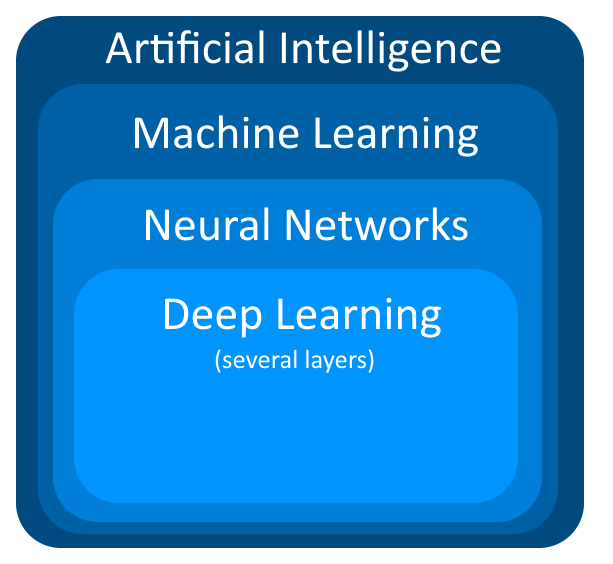
\includegraphics[width=6cm]{resources/ai.png}
	\caption{High level visual representation of what fields there are in the study of AI.}
	\label{fig:ai}
\end{figure}
\noindent The solution to having well trained models seems straight forward. We should use the vast amounts data from the edge devices to train a model that, in theory, should be fairly accurate. To do so, the users must give their data to a server so that the server can then train the model on the data that was just provided to it by the edge users. This trained model can then be used by everyone to predict unseen samples. But there are some more complications. Users may not want to share their data but still want the benefits of having a model trained on everyone's data. 
\subsection{Motivation}
Artificial Intelligence, specifically Machine Learning, is an idea that is taking the world by storm. A piece of software that would make machines autonomous. It was supposed to be better in every way, never getting tired, reaching at least the same competency levels as humans and quite possibly even better. It was hyped up to the point where the media started talking about AI putting people out of a job and eventually taking over the world. They even made far fetched references to the popular movie series Terminator.
\\\\
Needless to say, this is not accurate. The idea of a general purpose AI, formally called Artificial General Intelligence, is no where near attainable. Current AI applications are good at specific tasks, and only those tasks because they have a narrow scope. Even with their narrow scope there are more topics that need to be addressed, such as the security issues that arise with better AI systems. One can use AI to create cyberweapons that can be used for hacking and spreading misinformation. Along with cyberwarfare, AI can be used to make traditional weapons more lethal. For instance, drones are now being used to target specific areas (and people) using ideas like image classification. At first glance this seems like a good idea as it should result in less casualties. But, AI systems are not 100\% accurate so they could lead to an accidental strike. And if someone is able to hack into the system, they can make the drones target literally anything and anyone. Even in the right hands this technology can lead to disasters, let alone the wrong hands. Then there is the privacy aspect as well where people may not want to share their potentially sensitive private data under the fear that it can be misused. The idea of privacy will be the focus of this project.
\subsection{Privacy Concerns}
There are numerous examples where people may not want to share their personal data. For instance, for the training of a model that deals with predictive text, the input data would require essentially everything that a user may type into their device. It is pretty obvious to see why some people may not want to share the messages and other content that they type on their devices. It is a clear invasion of their privacy.
\\\\
Another application could be training on images for classification purposes. People may not want to share images, which may include sensitive images, that they have stored on their devices with a third party. This can be extended to an even more sensitive topic of medical imaging where people may not want to share something like the X-Rays of their bodies.
\\\\
In general, people are sceptical of sharing personal data. But there is still the need to train a model that has had exposure to as much data as possible. 
\subsection{Report Outline}
The need for privacy was the motivation behind the idea of Federated Learning which was an idea proposed by Google in 2016~\cite{mcmahan2016communication}. The idea of not having to share your data with someone else and yet still have the benefits of having a model that has exposure to their data will be the main point of interest in this report. 
\\\\
To start off, a brief overview of machine learning and neural networks will be provided in Sections~\ref{subsec:ml} and~\ref{sec:neuralnets} respectively. Then in Section~\ref{subsec:fedml} we will see how Google describe federated learning before discussing the design and implementation in Section~\ref{subsec:fedml-core}. Following Google's approach, several extended ideas based on weighted and selective approaches in a central and peer-to-peer environment will be discussed and their implementation explained in Section~\ref{sec:ext-ideas}. Along with that, outputs from the experiments to show how the extended ideas compare with Google's approach of federated learning and the traditional approach of machine learning in this context will be explained in Section~\ref{sec:experiments}. 
\section{Literature Review}
\subsection{Machine Learning}\label{subsec:ml}
Machine learning is a very broad field which includes a lot of different learning methodologies. Learning can take place in a supervised context where the dataset is labelled, or in an unsupervised context where the data is not labelled. 
\\\\
In unsupervised learning, the only input data are the features and there are no input-output mappings. The aim is to find structure within the dataset and can also be useful in finding anomalies in the dataset. The most well known algorithm for this purpose is k-means++ clustering.
\\\\
In supervised learning, the task is to learn a function that maps an input to an output, based on sample input-output pairs. In this project, the focus is on supervised learning where the aim is not to find structure within a dataset but rather trying to learn how to map the input data to a desired output. There are quite a few methods of finding the right function that fits the dataset, ranging from simple functions to very complicated functions.
\\\\
One of the simplest approaches for supervised learning is called Linear Regression, which aims to solve regression problems. The data that is provided to it are pairs consisting of input features (as a vector) and the desired output. Based on the set of input pairs provided, linear regression tries to find a linear function, which is a set of coefficients $\beta$ for all the features, that fits the dataset well. The set of input pairs provided is called the training set. To find the best possible function to fit the data, the idea of a loss function is used. This essentially says how distant the predictions are from the desired output. Loss in this case is usually mean squared error (MSE). The error $e$, is the difference between the actual value and the predicted value.
$$\mbox{MSE} = \frac{1}{n}\sum_{t=1}^{n}e_t^2$$
The values of $\beta$ that fit the dataset the best would be the one with the lowest value for MSE on the training data. A naive way to solve this problem would be to iterate over all the infinitely many $\beta$s and run predictions on the $n$ samples in the training set to give an output. We then use use the predicted output and the desired output to calculate the loss values for all the $\beta$ combinations. The $\beta$ values that give the lowest MSE value (loss) would be chosen as the solution. But there are more sophisticated methods of solving this such as gradient descent. The latter can intuitively be thought as taking, usually small, steps in the direction that reduces the loss. 
\\\\
Logistic Regression follows the same basic principle as linear regression but is used for classification purposes instead. Classification problems are about predicting if a sample belongs to a certain class or not. The input data for this is similar to linear regression with it being a pair of input features (as a vector) but the desired output being a label representing a class of objects (like ``dog''). Logistic regression still works off of building linear models using $\beta$ under the hood and predicts numbers that are probabilities of a certain input being part of a certain class. For the prediction, input features are passed through a sigmoid function $\sigma$ (also called the logit function) which outputs a number between 0 and 1, lets call this $h_\beta$. 
$$\sigma(z) = \frac{1}{1 + e^{(-z)}}$$
$$h_\beta(x) = \sigma(x\beta)$$
These numbers are interpreted as the probability of the input being part of a class, usually the positive class (a class which requires action and is labelled as 1). Based on the probability, the input is classified to a class $\hat{y}$.
$$\hat{y} = \left\{ 
    \begin{array}{ll} 
      0 & \mbox{if \textit{Prob}}(\hat{y} = 1 | x) < 0.5 \\
      1 & \mbox{if \textit{Prob}}(\hat{y} = 1 | x) \geq 0.5
    \end{array}
  \right.
$$
The idea of reducing the loss still applies, but a more complicated loss function is used in this case. Linear regression and logistic regression are both based off of a linear function so they cannot deal with complex data very well. Decision trees are an alternative that can better fit complex datasets and can be used for both regression and classification problems. They are more intelligible compared to other approaches. At a very high level, the structure of the tree dictates what path a sample input should take. A very simple decision tree can be seen in Figure~\ref{fig:decisiontree}. The inner nodes in the tree split the data based on conditions and the leafs represent the decisions made on the samples. A different loss function is used to optimise the answer.
\begin{figure}[H]
	\centering
	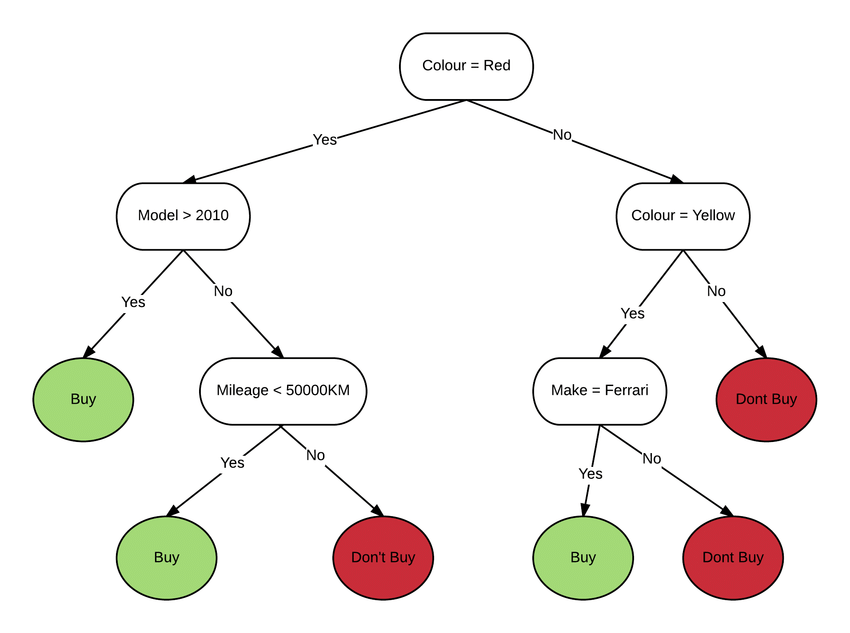
\includegraphics[width=8cm]{resources/decisiontree.png}
	\caption{A very simple decision tree~\cite{phdthesis}.}
\end{figure}\label{fig:decisiontree}
\noindent Neural networks have become the go to solution in recent times for pretty much all problems. They can cater to a wide range of problems, including very complex problems such as image classification, image localisation and natural language processing. They generally perform pretty well on those tasks too. There are also ways in which privacy concerns can be addressed when using neural networks. This is why they will be the only thing we use in this project.  
\subsection{Neural Networks}\label{sec:neuralnets}
Neural networks, as seen Figure~\ref{fig:ai}, are a subset of machine learning. Neural networks are not a new idea, they have been around for decades. But they only really took off in recent years with the emergence of better and more affordable hardware. The basic idea behind the workings of a neural network are quite straight forward. A model is defined and data is passed through it to make predictions. Then, based on the loss, some adjustments are made to the parameters learnt. This whole process is repeated by iterating over the dataset a set number of times during the training process. To start off, the idea of a neuron must be explained which are the basic building blocks of a neural network.
\\\\
\subsection{Neurons}
A neuron computes a weighted sum of its inputs, passes it through a function (called the activation function) and outputs a value to be used later. The inputs received are from either the input layer neurons or the hidden layer neurons. The activation function used below is a step function that outputs a $1$ if the weighted sum is more than a certain value ($0$ in this case), otherwise it outputs a $0$. The weight $w_0$ for the input data point labelled $1$ in Figure \ref{fig:neuron} is used to represent a bias. Because the input is $1$, multiplying it with a weight $w_0$ is guaranteed to give a value which will act as a number that is always used in the summing process later before the value is passed into the activation function. 
\begin{figure}[H]
	\centering
	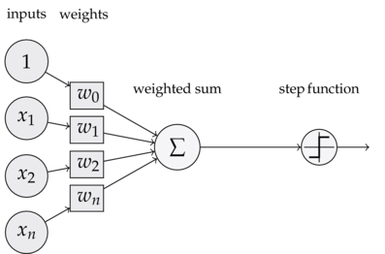
\includegraphics[width=6cm]{resources/neuron.png}
	\caption{Major components of a neuron~\cite{web:neuron}.}
	\label{fig:neuron}
\end{figure}
\noindent Note that, for brevity, the weighted sum can be written in a vectorised format. The weighted sum also includes $w_0$ which represents the bias.
$$w \cdot x \equiv \sum_j w_j x_j$$
$$  \mbox{output} = \left\{ 
    \begin{array}{ll} 
      0 & \mbox{if } w\cdot x \leq 0 \\
      1 & \mbox{if } w\cdot x > 0
    \end{array}
  \right.
$$
The activation function can be swapped out from the step function that was being used earlier with some other activation function such as ReLU (Rectified Logic Unit), sigmoid function, etc. ReLU takes the max of either 0 or the weighted sum and uses that as its output. This can be seen in equation~\ref{eq:relu}.
\begin{eqnarray}\label{eq:relu}
  \mbox{output}&=& \mbox{max}\left\{0,w\cdot x\right\}
\end{eqnarray}
\subsection{Architecture}\label{subsec:arch}
In a neural network, there are layers of such neurons. These are usually broken down in three parts, the input layer, the hidden layer(s) and then the output layer. The input layer is not actually a layer of neurons but rather just a representation of the input data as a layer that connects to the hidden layers. The hidden layers can contain any number of layers with any number of neurons for the layers.
\\\\
After the hidden layers is the output layer. This layer is responsible for outputting the predictions. The output layer usually has its own activation function which depends on the application, i.e., if it is a classification problem or a regression problem. Since this project focuses on multi-class classification problems, we will be using the softmax activation function for the output layer. 
\\\\
% start here-------------------
The layered structure described above is called the architecture of the model. Some of the common used architectures are densely connected layers (Section~\ref{subsubsec:dense}) and convolutional layers (Section~\ref{subsubsec:conv}). More information on the aforementioned and more architectures can be found in the book about Deep Learning by F. Chollet~\cite{deeplearning}.
\subsubsection{Dense}\label{subsubsec:dense}
These are one of the most straight forward architectures and are generally used as the output layer of most neural networks. They are quite useful when placed as the last few layers as well, especially for classification purposes. In these, all the neurons are connected to every neuron in the subsequent layer. The input for these layers are flattened data, which can be thought of as a list of input data where nested lists are not allowed. An example can be seen in Figure \ref{fig:densenet}. 
\begin{figure}[H]
	\centering
	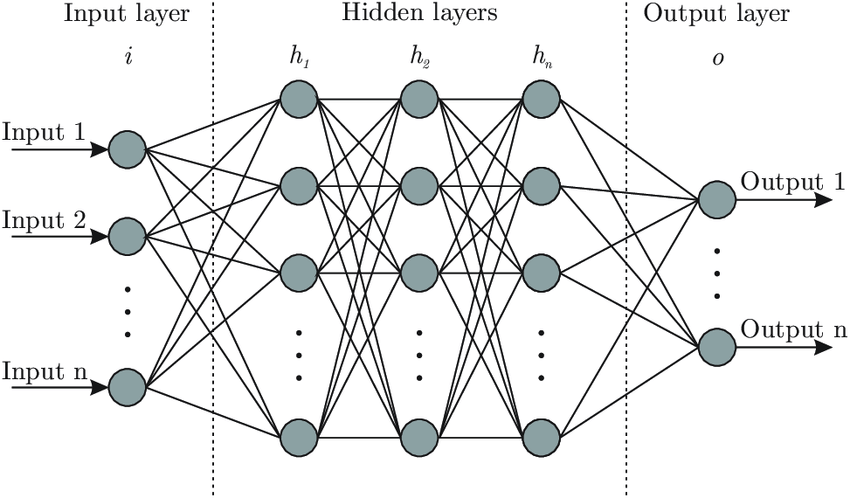
\includegraphics[width=8cm]{resources/densenet.png}
	\caption{Basic dense neural network~\cite{bre2018prediction}}
	\label{fig:densenet}
\end{figure}
\subsubsection{Convolutional}\label{subsubsec:conv}
These are more complicated than the previously mentioned dense layers. The input data here is structured and not flattened. Their basic idea is to find patterns in the input data and make them more abstract as the layer count increases. They indicate the presence of certain shapes. The more common use for convolutional layers is in image classification.
\\\\
A convolutional layer has a window (called the kernel) that is used to look over the input data and recognise patterns localised in that window. Every layer has a number of sub-layers which can be thought of as the number of patterns that the layer is trying to recognise and they are called the feature maps of the layer. For example if the depth is 3, the convolutional layer has 3 feature maps and will look at 3 kinds of patterns. The neurons in the following convolutional layer are connected to every neuron in the window of the previous layer, including the sub-layers as well. The set of weights that connect a neuron to the sub-layer neurons in the following layer are the same within the window. Figure \ref{fig:convnet} does a good job of giving a visual representation for the same.
\begin{figure}[H]
	\centering
	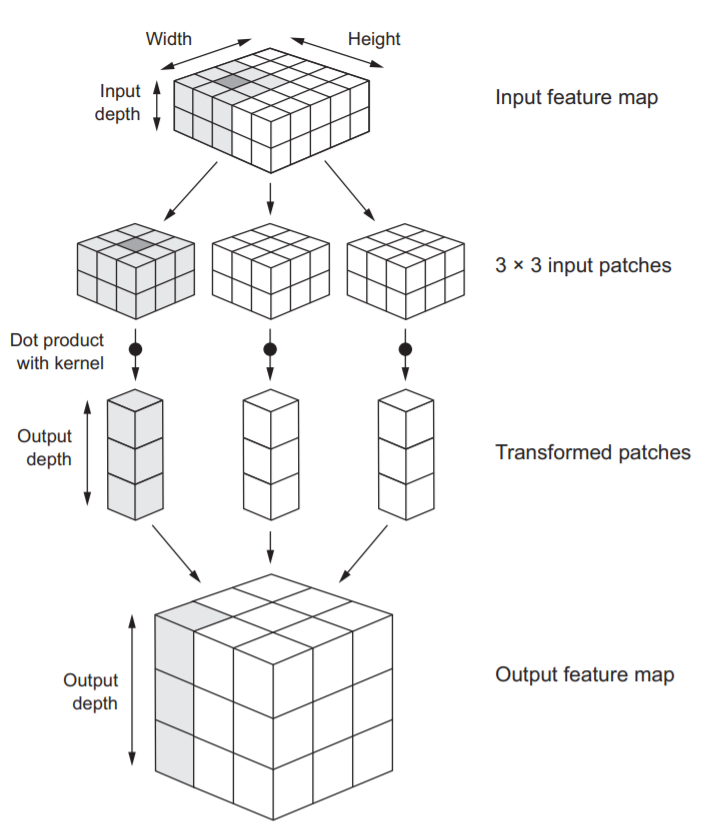
\includegraphics[width=8cm]{resources/convnet.png}
	\caption{How a convolution works~\cite{deeplearning}.}%page 125, chapter 5
	\label{fig:convnet}
\end{figure}
\noindent Convolutional layers are often followed by some maxpooling layers, which reduce the output size from the convolutional layers. This can be done for many reasons, such as saving memory and making the computations required less intensive. At the end of a series of convolutional layers, there is a series of dense layers that are used to give the predicted output(s). 
\clearpage
\subsection{Training}\label{subsec:training}
For a neural network to work, the weights with which the neurons are connected need to be tweaked and the process of doing so is called training the model. The model is trained on a training set, which is a subset of the whole dataset. Additionally, a validation set can be provided to see how the model performs on unseen data that is not the testing data. The progress is seen by comparing metrics for the model on both the training data and validation data over the course of the training. This is done to avoid leakage between the testing data and the training data. We will now go through the high level algorithm with which neural networks are trained. More information on this and the idea of neural networks can be found in the (online) book ``Neural Networks and Deep Learning, Michael A. Nielsen''~\cite{neuralnets} and the book ``Deep Learning with Python, Francois Chollet''~\cite{deeplearning}.
\\\\
The model is initialised with random weights before training begins. After that, the training data is then through the model to make predictions. These predictions are then compared with the actual values, and the loss is calculated using a loss function. For regression, mse is used and for classification sparse categorical crossentropy is used. The details in which they work are not required, but the idea of finding out how far off the predictions were from the actual value still holds. Using an methods like gradient descent or Adam (based on gradient descent and other methods, an algorithm called back propagation tweaks the weights in a way that would hopefully reduce the loss. These updates can be made based on every example, batches of examples or the entire dataset as a whole. Generally, the batched approach is taken and the entire dataset is broken down into batches of training data. 
\\\\
This whole process of predicting, calculating loss and tweaking the weights can be done several times by iterating over the whole training set several times. The number of times that the entire training set has been gone over is called the number of epochs that the network was trained on. This needs to be tweaked manually as it could lead to under-fitting or over-fitting the model. Which means, the model is too general or too specific, respectively, to be useful in actual usage.
\comment{\subsection{Differential Privacy (MIGHT OMIT THIS)}
linkage attacks, netflix and imdb data to identify
only good for large dataset, else bad 
	complex
	easier to do real data and anonymise 

deidentify data (outliers, fields)
 	
want to decouple learning about an individual and learning about the population

analysis output is not dependant on a particular individual and will be the sameif they are not incuded

adjacent dataset
	n+1 and n sized dataset, algo m
}
\subsection{Federated Machine Learning}\label{subsec:fedml}
Traditionally in ML, a server would have access to all the data. We call this server the central agent $C$. The data on the central agent is collected from a set of upto $n$ edge users which we call $U$. Each edge user i of U, represented as $U_i$, sends their data to the central agent. User $i$'s data is represented as $D_i$. Using all the data $C$ has access to, $D = \bigcup_{i=1}^{n} D_i$, it would train a single model $M$ which then anyone could then access to make predictions. 
\\\\
In Federated ML, $D_i$ remains with $U_i$ and instead only the weights of the user's model are shared. This means that at any give point, $C$ does not have access to any data $D_i$ from user $U_i$. By doing so, the privacy of the user's data is maintained. The training process in federated learning is performed on $U_i$'s device itself. To be able do so, an identical copy of $M$ is sent from $C$ to every participating $U_i$. Every $U_i$ then treats the model $M$ that they received as $M_i$. This means that every $M_i$ has the same architecture and the same randomly generated initial weights $W_i$. The weights are associated to the links that connect the neurons of the neural network as seen in Section~\ref{sec:neuralnets}.
\\\\
Once $U_i$ receives $M_i$, it can start training its $M_i$ on its local data $D_i$. The training process for $M_i$ generally starts based on certain conditions being met such as the device being plugged in for charging, WiFi connection, usage, etc. After the local training process for $U_i$ has been completed, $M_i$ would have new weights $W_i$. These weights would have been learnt and set such that they fit the user's $D_i$ relatively well. User $U_i$ then sends its learnt weights $W_i$ to $C$ for the averaging process to take place. The algorithm for the user side operations can be seen in Algorithm~\ref{algo:fedcore_user}. Instead of sending all the weights, an alternative would be to send only the changes made to the weights, which is what Google does.
\begin{center}\begin{algorithm}[H]
\texttt{\Fn{\FFedCoreUser{new\_weights}}{
	\If{new\_weights != None}{
		$M_i$.set\_weights(new\_weights)\\	
	}
	\For{\forcond{$e$}{$local\_epochs$}}{
		$M_i$.train()
	}
	$M_i$.send\_weights\_to\_server()
	return $M_i$.weights
	\caption{User side processing}\label{algo:fedcore_user}
}
}
\end{algorithm}\end{center}
\noindent When $C$ receives a set of upto $n$ weights $W_i$ from all the participating users, it uses them to calculate the average of the set of weights $W_{avg}$. The averaged weights $W_{avg}$ are then sent from $C$ to every $U_i$ in $U$. This can be seen in Algorithm~\ref{algo:fedcore_server}.
\begin{center}\begin{algorithm}[H]
\texttt{\Fn{\FFedCoreServer{$set_of_weights$}}{%\bigcup_{i=1}^{n}W_i
	$W_{avg}$ = average($set_of_weights$)\label{algo:fedcore_server:line:avg}\\
    send\_to\_all\_users($W_{avg}$)
    \caption{Server side processing}\label{algo:fedcore_server}
}
}
\end{algorithm}\end{center}
\noindent The averaging process is the reason why we need to use the same architecture for all models $M_i$. Without the same architecture, the shape for every $W_i$ would be different and therefore we would not be able to calculate an averaged $W_{avg}$ that would be compatible with every $M_i$. The averaging mentioned in in Algorithm~\ref{algo:fedcore_server} line~\ref{algo:fedcore_server:line:avg} is calculated by summing all received $W_i$ and dividing by the number of $W_i$ received, as seen in equation~\ref{eq:avg}.
\begin{equation}\label{eq:avg}
	W_{avg} = \frac{\sum_{i=1}^{n} W_i}{n}
\end{equation}
\noindent After receiving $W_{avg}$ from $C$, every $U_i$ replaces the weights $W_i$ for their $M_i$ with the new averaged weights $W_{avg}$. When the users have set the weights of their model $M_i$ to be $W_{avg}$, they can start the training process again. This back and forth of training, averaging and training again can take place several times. Every time $U_i$ trains their $M_i$ and shares their $W_i$ with $C$ to receive $W_{avg}$, it is called a $round$ of federated learning. After a few rounds, the resulting metrics can be pretty close to the metrics obtained with the traditional ML approach. Although, it must be noted that depending on the context the results may vary a lot and may require some changes as well. We will witness this in the experimentation section (Section~\ref{sec:experiments}) later in this report. 
\\\\
Algorithm~\ref{algo:fedcore} and Figure~\ref{fig:fedcore} provide a high level representation of the federated learning process. It starts off with $C$ sending the initial model to the all the users. This model is the same $M$ that was initialised with random weights in the traditional approach. It is provided to the algorithm as an input. After the users receive the model, for every round of federated learning, all the users set their weights to the new averaged weights (if provided), run local training and then share their current weights with $C$. $C$ would then calculate the new averaged weights and broadcast it to every $U_i$ and the whole process takes place again for a set number of rounds. The calls made in lines~\ref{algo:fedcore:line:user} and~\ref{algo:fedcore:line:server} are calls to algorithms~\ref{algo:fedcore_user} and~\ref{algo:fedcore_server} respectively.
\begin{center}\begin{algorithm}[H]
\Fn{\FFedCore{model}}{
	central\_agent.send\_to\_users(model)\\
    new\_weights = None\\
    \For{\forcond{round}{$rounds$}}{
	    weights = [ ]\\
        \For{\forcond{user}{$users$}}{
            user\_weights = central\_agent(new\_weights)\\\label{algo:fedcore:line:user}
            weights.add(user\_weights)
        }
        new\_weights = server(weights)\label{algo:fedcore:line:server}
    }
  \caption{Federated Learning Core overall algorithm}\label{algo:fedcore}
}
\end{algorithm}\end{center}
\begin{figure}[H]
	\centering
	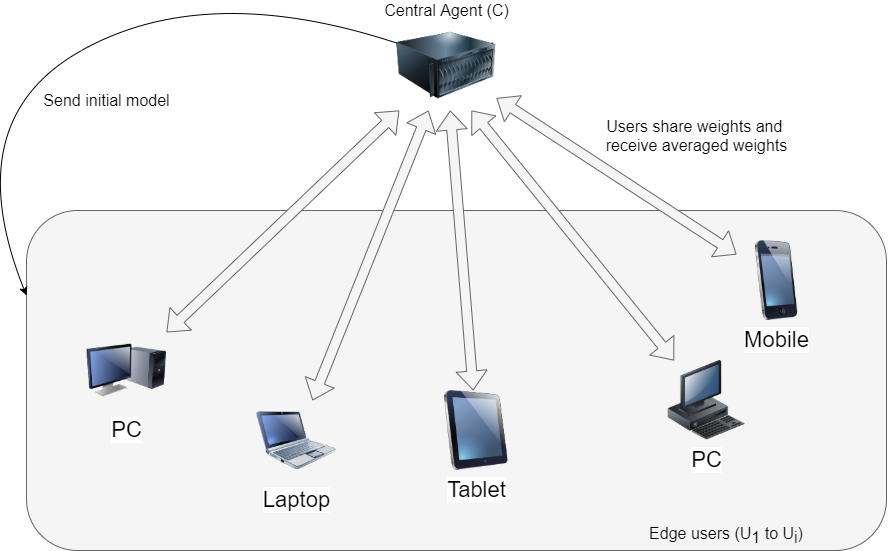
\includegraphics[width=\linewidth]{resources/fedml.png}
	\caption{Federated learning.}
	\label{fig:fedcore}
\end{figure}
\subsubsection{Benefits}
Federated machine learning has a few benefits. Firstly and most importantly, all the training takes places on the only the edge devices. This means that the users do not have to share their data with anyone. The only data they share are the parameters learnt from the training process that took place on their local data. And it is impossible to recreate the original data from just the parameters. Add to that the idea of Secure Aggregation~\cite{secagg} and one can very confidently say that the idea of privacy is held up to the highest standard. Secure aggregation is where the data is aggregated in stages. Instead of all averaging being done at the server where some data can possibly be reverse engineered, there are intermediary steps where the data is averaged and then the central agent finally averages those averages. Sometimes, noise is also added during this process. But we will not be focussing on secure aggregation in this project. 
\\\\
Secondly, the fact that all the training runs on edge devices means that there is no need for an investment in building a large training infrastructure by a company. The edge devices will do all the hard work of the model training and share the results which a central agent would then use quite trivially. So this is a better use of resources as a whole as idle devices would not just stay idle and would take part in the training process.
\subsubsection{Drawbacks}
As mentioned before, the federated approach can lead to similar performance as the the traditional approach. But this depends on the distribution of the data as we will see in later sections (\ref{subsec:imageset}. If the dataset amongst all the users is very similar, then the overall result of the federated process can be very similar to the traditional approach. But if the users have skewed datasets, as is often the case in real life, the traditional approach is generally better. It is a trade-off of privacy vs. model performance that must be decided upon when deciding between the federated approach and the traditional approach respectively.
\clearpage

\section{Core Design}
In this section, the design and implementation aspect of the basic approaches will be discussed before moving on to discussing the extended ideas explored in this project. 
\subsection{Non-Federated Learning}\label{subsec:non-fedml}
Before talking about federated learning, we first need to set in place the traditional machine learning approach. For this, the idea of an imaginary user is utilised. We refer to this user as the $global\_user$. The $global\_user$ assumes that we have access to data from every user. We set the metrics from this approach as \textit{the} benchmark to beat. If any federated approach can be close to these metrics, then we can say that we can preserve privacy whilst maintaining a similar level of performance.
\subsubsection{Design}
This approach is quite straight forward in terms of what is to be done. The data is readily available to be used, so the first first step is to pass the training data into the model for training. The second one is to record how well the model performs on the training and validation data for every epoch of training.
%approach involves finding a way to split the data, selecting a model, passing the data to the model for training and recording the metrics to analyse the performance of the model. 
\\\\
With the dataset readily available for use, we need to select a model that fits the dataset well. We will look at how to find a dataset specific model in Section~\ref{sec:experiments} where we perform experiments on different datasets. Given that the data and model are now ready to be used, we can pass the training data into the model to train it. The training process described in Section~\ref{subsec:training} is carried out and the model is trained on the training data for a number of epochs. To ensure that we can review the progress of the model, we also make sure that we evaluate the model between every epoch of training on the validation and testing data. This can then be plotted on a metric versus epoch graph to visualise the model's performance over time. For the final performance score of the model, we can evaluate the model after the training process has been completed on the completely unseen test data.
\subsubsection{Implementation}
With the approach being straight forward, its implementation is quite trivial. To be able to discuss the implementation, an overview of the technologies used in this project is required. The language of choice for this project was Python and the biggest reason for choosing it was the Keras~\cite{chollet2015keras} library for deep learning. In this project, it uses with TensorFlow as its back-end to perform calculations. Keras provides a user friendly API to use Tensorflow to build neural networks with ease in Python. We chose to use TensorFlow as Keras' back-end because we will be using TensorFlow Federated (TFF) in Section~\ref{subsec:tff} as a sanity check to confirm that our implementation of federated learning matches that of Google. TFF provides a framework which allows people to build a federated learning system without having to deal with the low level details. Another library used extensively was Matplotlib. Matplotlib is a Python library used for plotting graphs which. It allowed us to review the learning progress of the neural network and be able to compare the performance of different approaches explored in this project. Pandas and numpy were two more extensively used libraries that were used for data representation throughout the project.
\\\\
The model $M$ that is used here is initialised in Keras. The initialisation process is essentially selecting an architecture that works well on the dataset and then compiling it for further use, like training. Keras models require the input for the training process to be data in one of either two formats, pandas DataFrames or numpy arrays. We choose the latter as the way to store the data that we have to make it easier to pass data into the model for training and evaluation. Keras also requires the features of the data to be separate from the label associated with a sample. The low level control on the numpy arrays also allows us to perform more specific tasks, such as this separation of features and labels, on the dataset as and when required.
\\\\
To train the model, we use the API that Keras provides for its models. A method called \texttt{fit} is associated to the model object which is used to train the model. The arguments passed into the method are the training data, validation data, epochs and the batch size. The training data is used to train the model. The validation data is used to gain some insight into how the model performs on data that is not the training data. Epochs is the number which specifies the number of times the training process iterates over the entire training data. The batch size dictates the number of samples in the training data that must be processed before changes to the weights of $M$ can be made. A simple call to this method on the model object will result in our model being trained on the training data.
\\\\
We also need to record the performance of the model over time to be able to plot graphs using matplotlib. Keras, whilst training, maintains a history of the metrics obtained between epochs on the model object. Between epochs, the model is evaluated on the training and validation data, and the result is stored in a dictionary in the model object. This dictionary can be accessed to get what is essentially the progress report for the model on the validation and training data. We use this data to plot the graphs to see how well the model is performing. 
\\\\
\subsection{Federated Learning}\label{subsec:fedml-core}
With the non-federated learning approach in place, we can discuss the federated approach in a similar way. This approach is exactly as explained before in Section~\ref{sec:fedml} and as such, this section will not include a lot of details which were explained previously. 
\subsubsection{Design}
In any federated approach explored, there is an obvious need to simulate users that take part in the process. But there is no point in  implementing a network of users when the idea of users can be simulated on just one machine. These simulated users have one main goal, they must not be able to access data from other users. We needed to come up with a way to simulate users who only have access to their local data and their local model. In other words, a way where only $U_i$ can access $M_i$ and $D_i$. To do so, we chose an objected oriented approach where the users would be represented as objects $U_i$. These objects would contain all the information relevant to a given user and nothing more. This means that user object $U_i$ would have access to $M_i$ and $D_i$. It is to be noted that for a given dataset, all user models $M_i$ are the same as model $M$ which was selected for the $global_user$. 
\\\\
The core federated learning algorithm used here is the same as Google's algorithm~\ref{algo:fedcore} described in Section~\ref{subsec:fedml}. But it's design was altered just a little bit to allow us to review the progress of the federated learning process and accommodate our for choice of not representing $C$ as a distinct user. 
\\\\
The decision to not represent $C$ as an object was taken because its functionality could be incorporated in the logic of the algorithm itself. This is done by replacing line~\ref{algo:fedcore:line:server} in algorithm~\ref{algo:fedcore} by line~\ref{algo:fedcore_server:line:avg} in algorithm~\ref{algo:fedcore_server}. As for being able to review progress at the end, we had to store evaluation metrics of the model on the test data before and after the local training process. These evaluations were done during every round of federated training. We call these evaluations $pre\_fit$ and $post\_fit$ evaluations respectively. The $pre\_fit$ evaluations allow us to see the model's performance with the averaged weights and the $post\_fit$ evaluations allow us to see the model's performance with the weights after local training is performed. This helps us see how well the averaged weights and post training weights fit an arbitrary user $U_i$'s test data $D_i$. 
\\\\
We augment algorithms~\ref{algo:fedcore} and~\ref{algo:fedcore_user} to reflect these changes which results in algorithms~\ref{algo:fedcentral} and~\ref{algo:fedcentral_user}. The averaging in line~\ref{algo:fedcentral:avg} still uses equation~\ref{eq:avg}.
\begin{center}\begin{algorithm}[H]
\texttt{\Fn{\FFedCoreUser{new\_weights}}{
	\If{new\_weights != None}{\label{algo:fedcentral_user:line:if}
		$M_i$.set\_weights(new\_weights)\\	
	}
    evaluation = user.evaluate\_model()\\
	user.add\_pre\_fit\_evaluation(evaluation)\\
	\For{\forcond{$e$}{$local\_epochs$}}{
		$M_i$.train()
	}
    evaluation = user.evaluate\_model()\\
    user.add\_post\_fit\_evaluation(evaluation)\\ 
	\textbf{return} $M_i$.weights
	\caption{User side processing}\label{algo:fedcentral_user}
}
}
\end{algorithm}\end{center}
\begin{center}\begin{algorithm}[H]
\Fn{\FFedCore{model}}{
    send\_to\_users(model)\\
    new\_weights = None\\
    \For{\forcond{round}{$rounds$}}{
	    weights = [ ]\\
        \For{\forcond{user}{$users$}}{
           user\_weights = user(new\_weights)\\          
           weights.append(user\_weights)\\
        }
        new\_weights = average(weights)\label{algo:fedcentral:avg}
    }
  \caption{Federated Learning}\label{algo:fedcentral}
}
\end{algorithm}\end{center}
\noindent The algorithm starts off by sending the model $M$ to every user. Each user then refers to their model as $M_i$. Then, before the model is trained by the user, it is evaluated on the users test data and that information stored in the collection of $pre\_fit$ evaluations for the user. We can do the evaluation on test data without the fear of leakage because we do not use the results to make changes to the model. Every user $U_i$ then trains their model on their training data to get the updated weights $W_i$ for their $M_i$. After the training, the evaluation is conducted once again on the test data and then stored in the collection of $post\_fit$ evaluations. The updated weights $W_i$ are returned by every user and stored in the main algorithm. This set of weights is passed in to the averaging function that returns an average of the weights called $W_{avg}$. The averaging function is based on equation~\ref{eq:avg}. These weights are then passed onto the users in the next round of federated learning, where they initialise their models with the new averaged weights and conduct the whole process again. After a set number of rounds, the federated learning process ends. In this project, we decided to use a high number so we could observe how the process runs over a long period of time. 
\subsubsection{Implementation}
The first thing that had to be implemented was the User class. It is used to store all the data local to a user. Instances of this user class are used to represent an arbitrary user $U_i$. The data stored on $U_I$ includes the training, validation and test data, the model of the neural network and the history of the metrics obtained during the training of the model. The training, validation and test data are stored as numpy arrays. Numpy arrays were used over standard Python array lists because of their vectorised operations which make them faster and more concise than using Python's array based lists. Another reason to user numpy arrays was because of the fact that Keras models require their input to be numpy arrays or pandas DataFrames. Storing the data as numpy arrays standardises the structure of the object for use throughout the project and increases re-usability of the code. The Keras model is stored in $U_i$ as well along with the $pre\_fit$ and $post\_fit$ metrics which are stored in numpy arrays. The details of the completed class can be seen in Figure~\ref{fig:classes_user}. 
\begin{figure}[H]
	\centering
	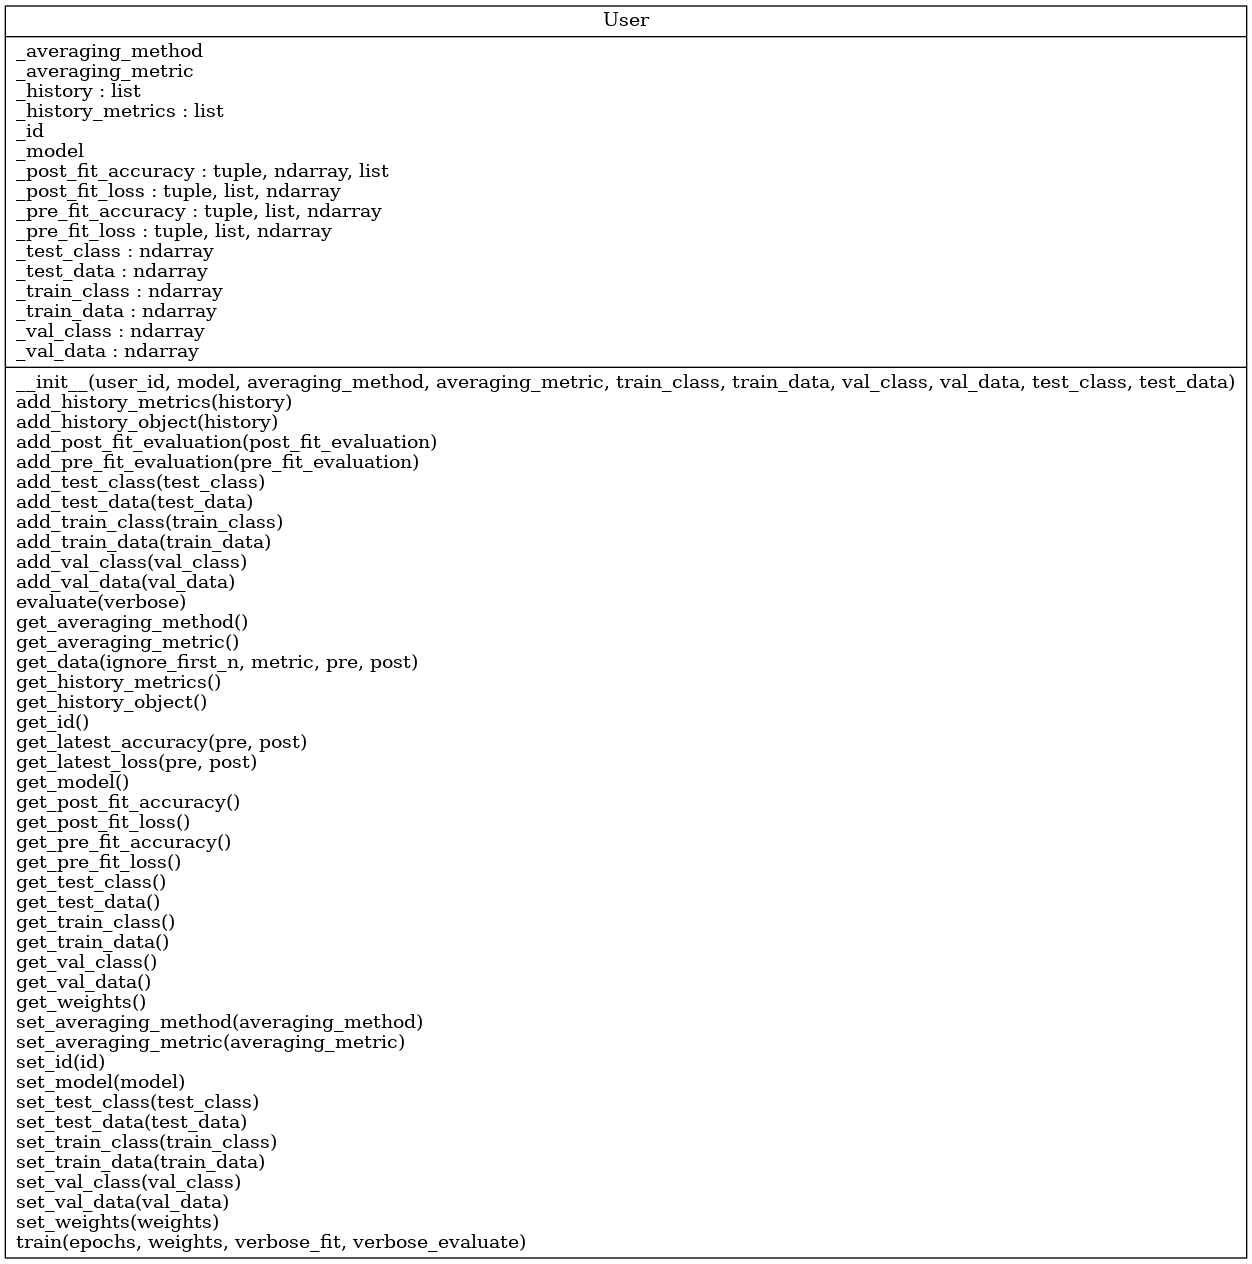
\includegraphics[width=\linewidth]{resources/classes_User.png}
	\caption{Methods and attributes of the User class.}
	\label{fig:classes_user}
\end{figure}
\noindent Then for every user in the dataset, we must instantiate a user object $U_i$ to represent them. The data relevant to the user is stored in this object after that. The details of this process will be explored in Section~\ref{sec:experiments}. After initialising the users, implementing the main algorithm was the next goal. 
\\\\
The algorithm starts off by sending $M$ to all the users which would ordinarily be done in a networked fashion but since we are using simulated users, a simple for loop suffices. In the loop, a copy of the compiled Keras model $M$ is stored in every $U_i$ which the users then refer to as $M_i$. After doing so, the federated learning process can begin. This process was implemented as a function, \texttt{train\_fed}, to increase re-usability throughout the project. This function would take in arguments such as \texttt{epochs}, \texttt{rounds} and more, to allow for flexibility in terms of how to run the training process. In it we conduct a set number of rounds of federated learning in which the training of the user's model and the sharing and averaging of the weights takes place.
\\\\
To train all the user models, we iterate over all the users and call the \texttt{train} method on every $U_i$. In the \texttt{train} method, we make use of the API Keras provides for its models. Using the \texttt{set\_weights} method of $M_i$, we can set the weights of the model to be the weights that we pass into the method. For the first round of federated learning, we do not set the weights to be anything new. But for subsequent rounds, the averaged weights $W_{avg}$ are passed into the \texttt{set\_weights} method which set the weight of $M_i$ to be $W_{avg}$. After doing so, the model is evaluated on the test data by using the \texttt{evaluate} method of $U_i$. This method intern uses the \texttt{evaluate} method provided by Keras to run evaluation on their models on give data, test data in our case. This data is then stored in the numpy arrays dedicated to storing $pre\_fit$ metrics such as \textit{accuracy} and \textit{loss}. Then a simple call to the \texttt{fit} method of the model will train it on the training data that we pass into the method for a given number of epochs. After the training, we once again call the \texttt{evaluate} method of $U_i$ to evaluate the model on the test data and record the evaluations in the numpy arrays. As mentioned before, Keras also maintains history of the evaluations during the training process in the model object. This history is reset every time the \texttt{fit} method is called. So, after every local training process we store the metrics from this history in $U_i$ as well in a Python list. We can use this information to plot more graphs and review the progress of the learning process, but this time on a more granular level because this is a history of \textit{epoch} evaluations. The $pre\_fit$ and $post\_fit$ evaluations we store are \textit{round based} evaluations.
\\\\
Once all the users have been trained, their weights need to be averaged. To make the averaging process more modular, an class dedicated to averaging was implemented. This class is called Average. The details of the final version of the Average class can be seen in Figure~\ref{fig:classes_average}.
\begin{figure}[H]
	\centering
	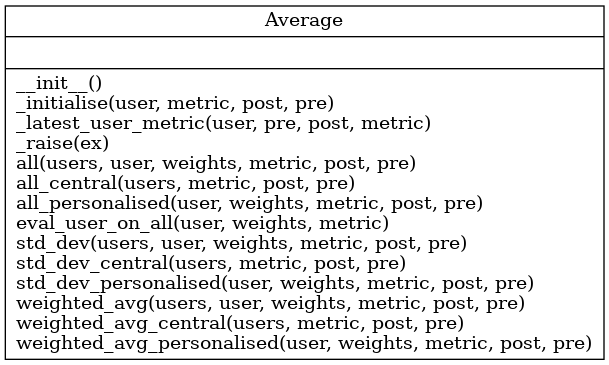
\includegraphics[width=10cm]{resources/classes_Average.png}
	\caption{Methods and attributes of the Average class.}
	\label{fig:classes_average}
\end{figure}
\noindent Residing in this class are static methods that deal with different kinds of averaging, one of which is the implementation of the averaging function in equation~\ref{eq:avg}. The method is provided with a reference to all $U_i$ in the form of a dictionary. With access to $U_i$ comes access to model $M_i$ for the user as well. The \texttt{get\_weights} method associated to $M_i$ is used to extract the weights $W_i$ from model $M_i$. This is done for every user and then those weights are used to calculate the averaged weights $W_{avg}$. Keras models store their weights as a list of numpy arrays. To be able to use numpy's quick calculations we cast the list into a numpy array of numpy arrays which is still referred to as $W_i$. We also initialise a numpy array full of zeros with the same shape as $W_i$ and name it $new\_weights$. This is used to collect the sum of all the weights as we iterate over all the users to calculate the average. As we iterate over the users, we use the \texttt{get\_weights} method to get the weights (which is a list of numpy arrays), cast it to a numpy array of numpy arrays and then add it to $new\_weights$. The shape of $new\_weights$ never changes throughout the whole process. This means that at the end of the loop we can divide $new\_weights$ by the number of users and get $W_{avg}$. $W_{avg}$ is then returned into the main function \texttt{train\_fed} where it will be fed back to all the users for the next round of federated learning where they initialise their models $M_i$ with weights $W_{avg}$. After a set number of federated learning rounds have been performed, we can stop the process and plot graphs from the metrics we had stored along the way. Our choice of choosing a high number of rounds lets us know at exactly what point the metrics start plateauing, and we can then say that training after that point is not necessary. 
\subsection{TensorFlow Federated}\label{subsec:tff}
In this section we will talk about simulating federated learning using TensorFlow Federated (TFF). The design aspect of this will not be discussed as it is the same as the federated approach we just discussed. Instead, we will focus on the implementation of federated learning using TFF. We implemented this approach for it to serve as a sanity check to see if our implementation as described in Section~\ref{subsec:fedml-core} is sound. 
\\\\
TensorFlow Federated is a framework for that allows for computation on decentralised data. TFF essentially has its own underlying language that can be accessed with Python. The building blocks of which are federated computations, which are computations that take place in a federated setting. TFF has two layers, the Federated Learning (FL) layer and the Federated Core (FC) layer. The Federated Learning layer allows high level plugging of Keras models into the TFF framework. We can perform basic tasks like the federated training process or evaluation without having to deal with the lower level concepts. The Federated Core layer provides us with low level control over the algorithms used in federated learning. In this section, we will be using the FL layer and not the FC layer as we do not need to implement custom algorithms. 
\\\\
TFF provides detailed documentation and tutorials on how to implement federated learning. The implementation here is based on those tutorials. We will assume that the dataset here is preprocessed and ready to be used, details on how this was achieved for experiments can be seen in Section~\ref{sec:experiments}. The basic idea is that every user's data is to be put into a Dataset object that is part of TensorFlow's data representation library \texttt{tff.data} and made into TensorFlow datasets for clients. A list of these, corresponding to every user, is used going forward in the training process and evaluation process. A model architecture is then defined using Keras, but unlike the other approaches we have seen so far, we do not compile the model. This is done at a later stage in the process. A function is defined that constructs and returns a Keras model. We call it \texttt{create\_model}. For models to be used in TFF, they need to be wrapped in a Model interface that is part of TFF's learning library \texttt{tff.learning}. This interface exposes methods that TFF needs to carry out training and other federated operations on the model in a federated setting. TFF will wrap the model for us by invoking a call to the function \texttt{tff.learning.from\_keras\_model}. We pass the non-compiled model from \texttt{create\_model} into this function, along with other parameters like the loss function, metrics functions and a sample of the dataset. The sample of the dataset is provided for initialisation purposes. This process of constructing the model and wrapping the model is placed into a function as well. We call this function \texttt{model\_fn}.
\\\\
We can now initiate the federated learning process with TFF. A simple call to the function \texttt{tff.learning.build\_federated\_averaging\_process} with \texttt{model\_fn} as the parameter constructs a Federated Averaging algorithm and packages everything into a \texttt{tff.utils.IterativeProcess} which we call \texttt{iterative\_process}. This constructs everything that needs to be done on the central agent and on the user's end, including compiling the model distributing them to users. It essentially implements everything that takes place in a round loop iteration in algorithm~\ref{algo:fedcore}. We can now initialise \texttt{iterative\_process} by calling the \texttt{initialize} method on it which returns the server state which we call \texttt{state}. A single round of federated averaging is performed by making a call to the \texttt{next} method on the initialised \texttt{iterative\_process} object. We pass \texttt{state} and the training data into the \texttt{next} method which returns the updated server state \texttt{state} and the metrics at the end of the round. The method call causes all the local 
ing on the simulated users, sharing and averaging of the weights and reinitialising the users models with the averaged weights to take place. Running the \texttt{next} method for a number of times representing the rounds of federated learning we want to perform. 
\\\\
At the end of the training, we must evaluate the model. For that we make a call to \texttt{tff.learning.build\_federated\_evaluation} and pass in the \texttt{model\_fn} we defined. This initialises the federated computations that need to take place for this process returns the corresponding federated computation object. We pass in the trained model and testing data into this to receive the evaluation of the model on the testing data. The trained model containing the averaged weights can be accessed from the server state that is returned after a round of federated learning. These metrics represent the performance of this implementation of federated learning using TFF. The comparison of the TFF implementation and our implementation of federated learning can be seen in Section~\ref{sec:experiments}. The results showed that the two implementation did not differ massively, which meant that our implementation was logically sound and that we could use it for further experiments.
\\\\
We decided not to use the TFF implementation because of the learning curve required in working with the FC layer of TFF. It was more intuitive to work with a sound implementation that we had built up from scratch instead of having to hack together our extended ideas using the TFF framework. 
\clearpage



\section{Extensions to Federated Learning}\label{sec:ext-ideas}
In this section, we introduce several extensions to Google's federated learning idea that we conceived in the course of this project. These extensions are based on different averaging methodologies in a central and peer-to-peer averaging context. We will also look at an idea where the users do not share their weights with anyone.
\subsection{Centralised Averaging}
Google's version of federated learning is implemented in the context of central averaging. This is where a \textit{central} agent $C$ handles the process of averaging the set weights sent from a set of users. In Google's approach described in Section~\ref{subsec:fedml-core} the averaging is done in a neutral way where every participating user's weights are weighed equally and they are all included in the averaging process. This was previously illustrated in equation~\ref{eq:avg}. We will now look at some ideas where that is not the case. 
\subsubsection{Weighted Average}\label{subsubsec:weighted-avg}
Our first extension is weighted averaging. In weighted averaging, the idea is to weigh the weights of certain users more than others in the averaging process. The criteria on doing so are the latest evaluations that the users obtain when evaluating their model on their validation data. The evaluations provided by user $U_i$ are referred to as $E_i$. Previously, the only thing that the users had to send to $C$ were their weights $W_i$. But now, the users must also send their evaluation $E_i$ to $C$, along with their weights $W_i$. This allows $C$ to make decisions on which weights should be weighted more when computing the averaged weights.
\\\\
For example, let us consider two users $U_x$ and $U_y$ with their latest evaluations being $E_x$ and $E_y$. If the value of $E_x$ is 100 and $E_y$ is 50, where higher is better, then $W_x$ will be weighted twice as much as $W_y$ in the weighted average $W_{avg}$. To achieve that, we compute the sum of $W_x \times E_x$ and $W_y \times E_y$ and divide it by $E_x + E_y$. This results in a weighted average $W_{avg}$ for users $U_x$ and $U_y$ where $W_x$ is weighted twice as much as $W_y$ in accordance with their respective evaluations. This can be generalised into an equation with $n$ users as seen in equation~\ref{eq:weighted-avg}.
\begin{equation}\label{eq:weighted-avg}
	W_{avg} = \frac{\sum_{i=1}^{n} \left({W_i \times E_i}\right)}{\sum_{i=1}^{n} {E_i}}
\end{equation}
In the case where the choice of metric is such that a lower value is better than a higher one, such as in loss, we replace $E_i$ by its inverse $\frac{1}{E_i}$ in equation~\ref{eq:weighted-avg}. If in this case $E_i$ is zero, then its inverse is not defined. There are several ways to deal with that, but in this project we chose to just use $10^{-6}$ as $E_i$ and then take its inverse. 
\\\\
The design of the federated learning process with weighted averaging is very similar to what is described in Section~\ref{subsec:fedml-core} with only a couple of changes. The first change is that the user must also share their latest evaluations along with their weights. We change algorithms~\ref{algo:fedcentral_user} and~\ref{algo:fedcentral} to algorithms~\ref{algo:fedcentral-weightedavg_user} and~\ref{algo:fedcentral-weightedavg} respectively to reflect this change.
\begin{center}\begin{algorithm}[H]
\texttt{\Fn{\FFedCoreUser{new\_weights}}{
	\If{new\_weights != None}{
		$M_i$.set\_weights(new\_weights)\\	
	}
    evaluation = user.evaluate\_model()\\
	user.add\_pre\_fit\_evaluation(evaluation)\\
	\For{\forcond{$e$}{$local\_epochs$}}{
		$M_i$.train()
	}
    evaluation = user.evaluate\_model()\\
    user.add\_post\_fit\_evaluation(evaluation)\\ 
	\textbf{return} $M_i$.weights, evaluation
	\caption{Central averaging user side processing}\label{algo:fedcentral-weightedavg_user}
}
}
\end{algorithm}\end{center}
\begin{center}\begin{algorithm}[H]
\Fn{\FFedCentral{model}}{
    send\_to\_users(model)\\
    new\_weights = None\\
    \For{\forcond{round}{$rounds$}}{
	    data = [ ]\\
        \For{\forcond{user}{$users$}}{
           user\_weights, user\_evaluation = user(new\_weights)\\
           data.append((user\_weights, user\_evaluation))\\
        }
        \# Below, different equations decide what kind of \\
        \# averaging takes place\\
        new\_weights = average(data)\label{algo:fedcentral-weightedavg:avg}
    }
  \caption{Central Federated Learning}\label{algo:fedcentral-weightedavg}
}
\end{algorithm}\end{center}
The second change is that we make line~\ref{algo:fedcentral-weightedavg:avg} in algorithm~\ref{algo:fedcentral-weightedavg} use equation~\ref{eq:weighted-avg} instead of equation~\ref{eq:avg}. Doing so successfully converts Google's federated learning process based on equal averaging into one that works on weighted averages instead.
\\\\
As for the \textit{implementation} of this idea, it was fairly trivial because of the way the framework was implemented in Section~\ref{subsec:fedml-core}. The only thing to be changed in the implementation was the averaging function. It had to be swapped out with a weighted averaging function that is in accordance with equation~\ref{eq:weighted-avg}. To do so, another static method is implemented in the class Average to compute the weighted average. This method is once again provided with a reference to all users in a dictionary data structure. With access to $U_i$ we also get access to its model $M_i$ and its latest evaluation $E_i$, both of which are stored in $U_i$. We start off by initialising a numpy array full of zeros with the same shape as $W_i$ and name it $new\_weights$. We use this to collect the sum of the weights as we iterate over all the users to calculate the weighted average. As we iterate though the users, we get the weights of the user's model by using the \texttt{get\_weights} method on $M_i$. We convert the returned weights $W_i$, a list of numpy arrays, into a numpy array of numpy arrays for quick calculations and concise code. We then retrieve $E_i$ to be multiplied with $W_i$. In the case where the metric for $E_i$ is accuracy, we perform a scalar multiplication of the weights with the accuracy. In the case where the metric for $E_i$ is loss, we perform a scalar multiplication of the weight with the inverse of the loss using $10^{-6}$ as the loss if it is zero. We store the resulting weights by adding them to $new\_weights$ in every iteration. The shape of $new\_weights$ never changes throughout the entire process. We also keep a sum of all the evaluations $E_i$ used, which we call $E_sum$. After iterating over all the users, we divide $new\_weights$ by $E_sum$ to get $W_{avg}$ and return it back to the main algorithm for the next federated learning round. Before returning $W_{avg}$, it is converted back into a list of numpy arrays. This process is in accordance with equation~\ref{eq:weighted-avg} which is used to calculate the weighted average.
\subsubsection{Selective Inclusion}\label{subsubsec:selective-inclusion}
In selective inclusion, the idea is to once again use the evaluations in the averaging process. But instead of using every user's weights in the averaging process, we only select a subset of the users that fit the criteria to be included in the averaging process. The averaging process used here is neutral and not weighted. The criteria to be included in the averaging process is that their evaluations are within a certain range which is considered to be acceptable. More specifically, their evaluations are at most one standard deviation worse than the mean of all the participating users. We chose this criteria because if a user's evaluations are worse than one standard deviation of the mean, the user is not doing as well as the other users. So their weights are not as valuable as the other users' weights. So we do not include them in the averaging process.  The averaged weights are then calculated from weights of the users who fulfil this criteria. Naturally, this approach requires the user $U_i$ to share their latest evaluation $E_i$ along with their weights $W_i$ to the central agent $C$ for averaging. Since this is already done in algorithms~\ref{algo:fedcentral-weightedavg_user} and~\ref{algo:fedcentral-weightedavg}, there are no changes required in the algorithms for this approach and we can continue to use those two algorithms here as well.
\\\\
Let us take an example to illustrate how this idea works with a user $U_x$. The evaluation on the validation data for $U_x$ is $E_x$ with the metric being accuracy. The mean and standard deviation for the metrics over all users $U$ is $\bar{E}$ and $\sigma$ respectively. The weights $W_x$ of user $U_x$ are included in the averaging process, if and only if $E_x$ is greater than or equal to $\bar{E}-\sigma$. If the criteria of $E_x >= \bar{E}-\sigma$ is not fulfilled, then $W_x$ is excluded from the averaging process. If $U_x$ is the only user to be excluded from the averaging, then the averaged weights are calculated by summing up the weights of all other users and dividing them by $n-1$. We subtract $1$ because $W_x$ is not included in the averaging process. This can be written in a generalised form as seen in equation~\ref{eq:selective-avg} which relies on equations~\ref{eq:selective-avg-mean} and~\ref{eq:selective-avg-stddev}.
\begin{equation}\label{eq:selective-avg-mean}
	\bar{E} = \frac{\sum_{i=1}^{n}{E_i}}{n}
\end{equation}
\begin{equation}\label{eq:selective-avg-stddev}
	\sigma = \sqrt{\sum_{i=1}^{n}{\frac{\left( {E_i - \bar{E}} \right)^{2}}{n}}}
\end{equation}
\begin{equation}\label{eq:selective-avg}
	W_{avg} = \frac{\sum_{i=1}^{n} \begin{cases}
		W_i, & \text{if }E_i>=\left(\bar{E}-\sigma\right)\\
		0,   & else
	\end{cases}}
	{\sum_{i=1}^{n} \begin{cases}
		1, & \text{if }E_i>=\left(\bar{E}-\sigma\right)\\
		0,   & else
	\end{cases}}
\end{equation}
\\\\
In the case where the evaluation metric is loss, where a lower number is better, we need to make some changes to the equation. Equation~\ref{eq:selective-avg} caters to a metric where a higher value is better. To make it work for loss, the criteria must be changed from $E_i >= \bar{E}-\sigma$ to $E_i <= \bar{E}+\sigma$ and then it will work for a metric where a lower value is better.
\\\\
The \textit{implementation} of this idea is once again made trivial by the fact that the only change from the weighted average approach is the need for a new averaging function which conforms with equation~\ref{eq:selective-avg}. To do so, a static method implementing equation~\ref{eq:selective-avg} is added to the the Average class. The method is given a reference to all the users objects in a dictionary data structure. With access to $U_i$ comes access to all the data stored in $U_i$ as well, such as the model $M_i$ and latest evaluation $E_i$. We initialise a numpy array full of zeros with the same shape as the weights $W_i$. This is referred to as $new\_weights$ and is used to collect the sum of the weights from users who fulfil the inclusion criteria. We also maintain a counter $contributers$ to count the number of users contributing to the averaging process by fulfilling the criteria. As this approach requires the mean $\bar{E}$ and standard deviation $\sigma$ of all the evaluations $E$ from all the users $U$, we must first compute these values. To do so, we iterate over all the users and collect their $E_i$ into a numpy array called $E$. Then we use the API that numpy provides on its arrays to calculate the $\bar{E}$ and $\sigma$. Calling the function \texttt{mean} on the numpy array of all evaluations $E$ returns the mean value of $E$. Similarly, calling the function \texttt{std} on $E$ returns the standard deviation in $E$. One we have all this data ready, we once again iterate over the users in a loop where we check if $U_i$ satisfies the criteria of $E_i >= \bar{E}-\sigma$ in the case where the metric being used is accuracy. In the case of the metric being loss, we use $E_i <= \bar{E}+\sigma$. If the user satisfies the criteria, we add their weights $W_i$ to $new\_weights$ and increase $contibuters$ by one. To get $W_i$, we use the \texttt{get\_weights} method associated with the Keras model $M_i$. This returns a list of numpy arrays which we once again convert into a numpy array of numpy arrays for quick calculations and concise code. The shape of $new\_weights$ never changes in this whole process. At the end of the loop, we divide $new\_weigths$ by $contributers$ to get the averaged weights $W_{avg}$ and return it to the main algorithm for use in subsequent federated learning rounds. Before returning $W_{avg}$, it is converted into a list of numpy arrays.

\subsection{Peer to Peer}
In this section we will explore another one of our extensions to federated learning, this time one that makes it behave in a peer-to-peer way. Previously, the users would send their weights and evaluations to a central agent $C$ that would average their weights and send the averaged weights back to all the users. The averaging is based on the averaging methodology being utilised by $C$. The averaged weights are then used by the users in their models for the next round of federated learning. But in a peer-to-peer context, the averaging process takes place on every user's device itself instead of $C$. Every user $U_i$ in $U$ sends its weights to every other user in $U$ which means that every user $U_i$ has access to the weights from every user in $U$. We call this set of weights received from other users $W_{others}$. $U_i$ then performs evaluations locally using its own local validation data on its own model $M_i$ and on models initialised from every weight from the set $W_{others}$. This way it can emulate models that the other users have learnt. Doing so, $U_i$ can check how relevant everyone else's models are for its own data and take appropriate action depending on the averaging methodology being used. The evaluations obtained from this process are then used in the averaging process by $U_i$ to calculate $W_{avg}$. This $W_{avg}$ is used in the next round of local learning by $U_i$. It is not shared with any other users. As $W_{avg}$ is now specific to $U_i$, we call it $W_{i,avg}$. 
\\\\
We alter algorithms~\ref{algo:fedcentral_user} and~\ref{algo:fedcentral} to reflect these changes which results in algorithms~\ref{algo:fedp2p_user} and~\ref{algo:fedp2p} respectively. 
\begin{center}\begin{algorithm}[H]
\texttt{\Fn{\FFedCoreUser{set\_of\_weights}}{
	\If{set\_of\_weights != None}{
	    new\_weights = local\_average(set\_of\_weights)\\\label{algo:fedp2p_user-localavg}
		$M_i$.set\_weights(new\_weights)\\	
	}
    evaluation = user.evaluate\_model()\\
	user.add\_pre\_fit\_evaluation(evaluation)\\
	\For{\forcond{$e$}{$local\_epochs$}}{
		$M_i$.train()
	}
    evaluation = user.evaluate\_model()\\
    user.add\_post\_fit\_evaluation(evaluation)\\ 
	\caption{Peer-to-peer user side processing}\label{algo:fedp2p_user}
}
}
\end{algorithm}\end{center}
\begin{center}\begin{algorithm}[H]
\Fn{\FFedPTP{model}}{
    send\_to\_users(model)\\
    set\_of\_weights = None\\
	\For{\forcond{round}{$rounds$}}{
    	\For{\forcond{user}{$users$}}{
           user(set\_of\_weights)\\
        }
	    set\_of\_weights = [ ]\\
	   	\For{\forcond{user}{$users$}}{
			set\_of\_weights.append(user.weights)
        }
    }
  \caption{Peer-to-Peer Federated Learning}\label{algo:fedp2p}
}
\end{algorithm}\end{center}
\noindent Algorithm~\ref{algo:fedp2p} is a simulation of the peer-to-peer communication that would take place in a real world scenario where the users would broadcast their weights to one another. In the simulation, the algorithm acts as a coordinator for the process and takes care of sharing every user's weights with all users by collecting every user's weights and sending the set of weights to everyone. The algorithm starts off by sending all the users in $U$ the model $M$ that they will be using in this process. Then, for every round of federated learning, we start off by training all the users which is illustrated in algorithm~\ref{algo:fedp2p_user}. In this process, if the algorithm provides a set of weights to a user $U_i$, $U_i$ will calculate the averaged weights based on the local averaging methodology and then initialise its model with the newly computed averaged weights. The averaging will be discussed more in depth in the following section. If no weights are provided to the user, then the weights of the user's model are not changed. The model is then evaluated on the $U_i$'s local validation data and the evaluation results are stored in the $pre\_fit$ evaluations. After doing so, the model is trained for a number of epochs and then once again evaluated on the $U_i$'s local validation data and the evaluation results are stored in the $post\_fit$ evaluations. After the training process, all the weights from the users are collected and sent to every user in the next round of federated learning. When the next round of federated process begins, the whole process repeats once again. We do this for a set number of federated learning rounds.
\\\\
For the averaging process, $U_i$ can utilise the \textit{weighted average} or \textit{selective inclusion} methodology. The standard unbiased averaging, such as the one Google proposed, makes no difference in this context. Google's approach is where the weights are simply summed up and divided by the number of users participating to get the averaged weights, as in equation~\ref{eq:avg}. In a peer-to-peer context, if every user were to do carry out that process, they would all end up with the same $W_{avg}$. This $W_{avg}$ would also be the same as the one provided by $C$ in the standard central federated learning approach. This is why using Google's standard averaging federated learning in a peer-to-peer context makes no difference, as the results would the same if it was being done in a peer-to-peer context or a central context.
\\\\
The \textit{implementation} of this framework requires minimal changes with respect to the implementation of the central approach. The changes in implementation to cater to algorithms~\ref{algo:fedp2p_user} and~algorithms~\ref{algo:fedp2p} will be explained here. After the \texttt{train} method is called on every $U_i$, we iterate over all users again and create a dictionary mapping of user ID to their weights such that $U_i$'s ID $i$ points to $W_i$. User ID $i$ can be accessed from $U_i$ by using the \texttt{get\_id} method. We call this dictionary $id\_to\_weights$. This dictionary is then passed into the \texttt{train} method of $U_i$ in the next round of federated learning instead of the averaged weights which is a list of numpy arrays. In the \texttt{train} method of $U_i$, we now also have a check to see if the weights provided are in a dictionary data structure. If so, then the peer-to-peer learning process is being used and local averaging must be performed. So the dictionary is then passed into a method which is part of the class Average to compute the averaged weights $W_{i,avg}$ for $U_i$. This method is specific to the averaging methodology and will be explained in the following sections. After the local averaging method returns $W_{i,avg}$, the \texttt{set\_weights} method is used to set the weights of $M_i$ before local training commences. 
\subsubsection{Weighted Average}
In this section we discuss how federated learning with weighted averaging can be carried out in a peer-to-peer context. The generic peer-to-peer federated learning framework is made up of algorithms~\ref{algo:fedp2p_user} and~\ref{algo:fedp2p}. Line~\ref{algo:fedp2p_user-localavg} in algorithm~\ref{algo:fedp2p_user} is where the local weighted averaging process takes place. Weighted averaging in the context of a central agent is described in Section~\ref{subsubsec:weighted-avg}. The peer-to-peer version is very similar to what is described there. The basic idea still remains the same. We wish to weigh the weights of certain users higher than the others in the averaging process. But this decision is now taken by every user $U_i$ independently and based on evaluations made on $U_i$'s local validation data.
\\\\
For example, let us take a user $U_x$ with model $M_x$ and weights $W_x$. As per the peer-to-peer framework $U_x$ receives weights $W_y$ and $W_z$ from $U_y$ and $U_z$ respectively. The criteria for $U_x$'s weighting of $W_x$, $W_y$ and $W_z$ in the weighted averaging process is based on the individual evaluations of models initialised with the aforementioned weights on $U_x$'s validation data. $U_x$'s evaluation of $M_x$ with $W_x$ on its local validation data is $E_{x,x}$. To evaluate $W_y$, $U_x$ initialises $M_x$ with $W_y$ and evaluates it on its own validation data. We call this evaluation $E_{x,y}$. The same procedure is followed with $W_z$ to obtain $E_{x,z}$. By $U_x$ always performing the evaluations on its own validation data, $U_x$ can see how relevant a certain user's weights are with regards to its own local validation data. The best evaluation is the most relevant to $U_x$'s data and therefore the weights corresponding to that evaluation should be weighted higher than the others. It is very likely that $W_x$ will be weighted the highest as it has been trained on $U_x$'s training data which shares characteristics with its validation data. All the weights and evaluations are then used to calculate the weighted average as per equation~\ref{eq:weighted-avg}. The changes required based on the metric choices still apply. In the case where the choice of evaluation metric is such that a lower value is better than a higher one, such as in loss, we replace $E_{i,j}$ by its inverse $\frac{1}{E_{i,j}}$ in equation~\ref{eq:weighted-avg}. If $E_{i,j}$ is zero for such a case, then its inverse is not defined. As mentioned before, we then choose to use $10^{-6}$ as $E_{i,j}$ and then use its inverse in the process. This weighted average is specific to $U_x$ so we call it $W_{x, avg}$. Users $U_y$ and $U_z$ carry out the same process locally as well to get their own weighted averages, $W_{y, avg}$ and $W_{z, avg}$ respectively. Every user then sets their local models to be initialised with their respective weighted average to carry out local training for that round of federated learning. This process is repeated for every round of federated learning.
\\\\
The \textit{implementation} of this idea required us to add more static methods in the Average class. The main method that calculates the weighted average, as seen in line~\ref{algo:fedp2p_user-localavg} in algorithm~\ref{algo:fedp2p_user}, is named \texttt{weighted\_avg\_personalised} and is provided with the dictionary of weights $id\_to\_weights$ as one of its parameters. This method starts off by calling the another static method of class Average, named \texttt{eval\_user\_on\_all}, whose aim is to evaluate models initialised by all available weights on the current user's validation data. This method is provided with an object reference to the current user $U_i$ and the dictionary of weights $id\_to\_weights$. It starts off by storing the original weights of $M_i$, $W_i$, in a temporary  variable $original$ for future use. Another dictionary is also initialised using the keys from $id\_to\_weights$. We name this dictionary $id\_to\_evals$. Its aim is to store and map the user ID $j$ to the evaluations of the model initialised with $W_j$ on $U_i$'s validation data. This is done for every user's weights. It must be noted that only in this simulation do we know the user IDs that are associated with the weights. In a real world scenario these weights would be anonymous. We then iterate over all the weights $W_j$ in $id\_to\_weights$. For every iteration, we set the weights of $M_i$ to be $W_j$ using the \texttt{set\_weights} method that Keras provides for its models and then call the \texttt{evaluate} method on $U_i$. This, as mentioned before, evaluates $M_i$, which now hosts $W_j$ for its weights, on $U_i$'s validation data and returns the evaluation $E_{i,j}$. $E_{i,j}$ is essentially indicates how well $W_j$ works on $U_i$'s validation data. We then store a mapping of $j$ to $E_{i,j}$ in the $id\_to\_evals$ dictionary. After iterating over all weights and obtaining all the evaluations, we set the weights of $M_i$ to be $original$, which resets $U_i$ to have its original model weights. Then the dictionary $id\_to\_evals$ is returned to \texttt{weighted\_avg\_personalised}.
\\\\
In \texttt{weighted\_avg\_personalised}, we now initialise a numpy array full of zeros with the same shape as $W_i$ and name it $new\_weights$. We use this to collect the sum of the weights as we iterate over every weight $W_j$ in $id\_to\_weights$ once again to calculate the weighted average. We also initialise a variable $sum$ to zero which is used to keep a sum of the evaluations for use later in the averaging process. For every iteration, we convert $W_j$ to be a numpy array of numpy arrays instead of the list of numpy arrays default structure. This is done to have succinct code and efficient calculations. Then we fetch the evaluation $E_{i,j}$ for $U_j$'s weights from $id\_to\_evals$ by providing $j$ as the key. If accuracy is the metric that is being used, then we can use $E_j$ directly. But if loss is being used, we use the inverse of $E_{i,j}$, $\frac{1}{E_{i,j}}$, as $E_{i,j}$ instead. If $E_{i,j}$ is zero in such a case, then its inverse is not defined. So as mentioned before, we choose to just use $10^{-6}$ as $E_{i,j}$ and then use its inverse in the process. We add $E_{i,j}$ to $sum$ and we add $W_j \times E_{i,j}$ to $new\_weights$ to update the summed values in every iteration. After iterating through all the weights, we divide $new\_weights$ by $sum$ to get the weighted average $W_{i,avg}$ for $U_i$, in accordance with equation~\ref{eq:weighted-avg}. This $W_{i,avg}$ is converted into a list of numpy arrays and is then used by $U_i$ to initialise its $M_i$ using the \texttt{set\_weights} for the next round of federated learning. 
\subsubsection{Selective Inclusion}
In this section we discuss how federated learning with selective inclusion in the averaging process can be carried out in a peer-to-peer context. We will once again utilise the previously described generic peer-to-peer federated learning framework. This framework is made up of algorithms~\ref{algo:fedp2p_user} and~\ref{algo:fedp2p}. Line~\ref{algo:fedp2p_user-localavg} in algorithm~\ref{algo:fedp2p_user} is where the local selective inclusion averaging process takes place. The idea behind this averaging methodology in the context of a central agent is described in Section~\ref{subsubsec:selective-inclusion}. The peer-to-peer version is very similar to what is described there. The basic idea of excluding users from the averaging process based on the evaluation still remains. But this decision is now taken by every user $U_i$ independently and based on evaluations made on $U_i$'s local validation data.
\\\\
For example, let us take a user $U_x$ with model $M_x$ and weights $W_x$. As per the peer-to-peer framework $U_x$ receives weights $W_y$ and $W_z$ from $U_y$ and $U_z$ respectively. The criteria for $U_x$ to include any of the weights $W_x$, $W_y$ and $W_z$ in the averaging process is based on the individual evaluations of models initialised with the aforementioned weights on $U_x$'s validation data. $U_x$'s evaluation of $M_x$ with $W_x$ on its local validation data is $E_{x,x}$. To evaluate $W_y$, $U_x$ initialises $M_x$ with $W_y$ and evaluates it on its own validation data. We call this evaluation $E_{x,y}$. The same procedure is followed with $W_z$ to obtain $E_{x,z}$. By $U_x$ always performing the evaluations on its own validation data, $U_x$ can see how relevant a certain user's weights are with regards to its own local validation data. In selective inclusion, as per equation~\ref{eq:selective-avg}, the weights included in the averaging process need to have evaluations better than a threshold value. In the case where the evaluation metric is such that a higher values are better, like with accuracy, the condition to be fulfilled is $E_{i,j} >= \bar{E_i}-\sigma$ where $\bar{E_i}$ is the mean and $\sigma$ is standard deviation of all evaluations for user $i$, $E_i$. In the the case where the evaluation metric is such that lower values is better, like with loss, the condition is $E_{i,j} <= \bar{E_i}+\sigma$. The weights from corresponding evaluations that satisfy the condition are included in the averaging process. It is very likely that $W_x$ is included in the averaging process as it has been trained on $U_x$'s training data which shares characteristics with its validation data. This average based on selective inclusion is specific to $U_x$, so we call it $W_{x,avg}$. Users $U_y$ and $U_z$ carry out the same process locally as well to get their own local averages, $W_{y,avg}$ and $W_{z,avg}$ respectively. Every user then sets the weights of their local models to be their respective averages before carrying out local training for that round of federated learning. This process is repeated for every round of federated learning.
\\\\
The \textit{implementation} of this approach is very similar to what was previously explained in the peer-to-peer version of weighted averaging. We implement a static method in the Average class and name it \texttt{std\_dev\_personalised}. This method implements the selective inclusion averaging process in accordance with equation~\ref{eq:selective-avg}. To do so, the method is provided with the dictionary of weights $id\_to\_weights$ as one of its parameters. The method's usage can be seen in line~\ref{algo:fedp2p_user-localavg} of algorithm~\ref{algo:fedp2p_user}. This method, when invoked by user $U_i$, starts off by calling another static method of the Average class called \texttt{eval\_user\_on\_all}. The aim of this method is to evaluate models initialised by all available weights on the current user's validation data. As described in the previous section, this method returns a dictionary called $id\_to\_evals$. This dictionary stores the mapping of an arbitrary user $U_j$'s user ID $j$ to the evaluations of the model initialised with $W_j$ on the current user $U_i$'s validation data. The implementation of this method is described in the previous section. The values in the key-value pairs of dictionary $id\_to\_evals$ are the evaluations which we will refer to as $E$. We obtain $E$ by calling the \texttt{values} method on the Python dictionary object and cast the returned values object into a numpy array of evaluations. Doing so allows us to calculate the mean $\bar{R}$ and standard deviation $\sigma$ of $E$ trivially by making calls to the \texttt{mean} and \texttt{std} methods respectively on the numpy array of evaluations $E_i$. After doing so, we initialise a numpy array full of zeros with the same shape as $W_i$ and name it $new\_weights$. We use this to collect the sum of the weights. A variable named $contributers$ is also initialised to zero which is used to keep a track of count of users that satisfy the inclusion condition. This is used later when calculating the average. We then iterate over all the evaluations $E_{i,j}$ stored in $id\_to\_evals$ and check if the relevant conditions are being satisfied. In the case of the metric being accuracy, the condition is $E_{i,j} >= \bar{E_i}-\sigma$ and in the case of the metric being loss, we use $E_{i,j} <= \bar{E_i}+\sigma$. If the evaluation satisfies the condition, we add the weights corresponding to user ID $j$, $W_j$, to $new\_weights$ and increase $contibuters$ by one. User ID $j$ is used as the key to index into the dictionary $id\_to\_weights$ which returns $W_j$, the weights of $U_j$. We convert $W_j$ to be a numpy array of numpy arrays instead of the list of numpy arrays default structure. This is done to have succinct code and efficient calculations. After iterating through all the evaluations, we divide $new\_weights$ by $contributers$ to get the averaged weights $W_{i,avg}$ for $U_i$. This averaging process is in accordance with equation~\ref{eq:selective-avg}. This $W_{i,avg}$ is then converted into a list of numpy arrays and returned to the user. $U_i$ uses $W_{i,avg}$ to initialise its $M_i$ using the \texttt{set\_weights} for the next round of federated learning. 
\subsection{Localised Training} %local only
In this section, we describe the idea of localised training. With localised training, the users do not share their weights at all and keep training their model on their local training data. This is equivalent to every user performing non-federated learning locally, as described in Section~\ref{subsec:non-fedml}. Non-federated learning is one of the baselines that we use where a single model is learnt from all the available data. This approach is similar to that but where every user learns a model and the available data is only their own local data. This acts as another baseline that we can use to see how well users perform when only training with their local data.
\\\\
The upside to this idea is that the parameters that the user's model learns have more relevance to the user's local data. In theory, this should make the local predictions for a user better as the locally learnt parameters are not contaminated by the parameters from other users. That being said, if a wildly different prediction is attempted on the user's model, the chances of the prediction being unreliable are very high. This is because the user does not benefit from the knowledge that the other users have learnt in their parameters, so the scope of learning is narrower. For example, in a classification problem, if a user $U_i$ only has pictures of different breeds of dogs, then after localised training the model will be able to classify the different breeds of dogs fairly well. But if $U_i$ asks for an image of a cat to be classified, then the system would not be able to give a reliable prediction for the cat and possibly misclassify it as a breed of dog. This is because the system has not been exposed to images other than that of dogs, so it lacks the knowledge of classifying anything that is not a dog.
\\\\
The design for this idea is based off of the central federated learning framework that is laid out in algorithms~\ref{algo:fedcentral_user} and~\ref{algo:fedcentral}. We change algorithm~\ref{algo:fedcentral} such that we no longer provide user $U_i$ with new weights from $C$ and we change algorithm~\ref{algo:fedcentral_user} to show that no new weights are being set on the user's side. Only training of the model takes place on the user's side. As a result, we get algorithms~\ref{algo:fedlocal_user} and~\ref{algo:fedlocal}.
\begin{center}\begin{algorithm}[H]
\texttt{\Fn{\FFedCoreUser{}}{
    evaluation = user.evaluate\_model()\\
	user.add\_pre\_fit\_evaluation(evaluation)\\
	\For{\forcond{$e$}{$local\_epochs$}}{
		$M_i$.train()
	}
    evaluation = user.evaluate\_model()\\
    user.add\_post\_fit\_evaluation(evaluation)\\ 
	\textbf{return} $M_i$.weights
	\caption{Local training user side processing}\label{algo:fedlocal_user}
}
}
\end{algorithm}\end{center}
\begin{center}\begin{algorithm}[H]
\Fn{\FFedLocal{model}}{
    send\_to\_users(model)\\
    \For{\forcond{round}{$rounds$}}{
        \For{\forcond{user}{$users$}}{
           user\_weights = user()\\          
        }
    }
  \caption{Local Learning in the federated framework}\label{algo:fedlocal}
}
\end{algorithm}\end{center}
The procedure still follows the idea of training all users over rounds of federated learning, but without actually sharing weights between the users. For every round of federated learning, all the users train their models for a number of local epochs. The users also keep a note of the evaluations of their models on their local test data before and after the local training process takes place. This data is called the the $pre_fit$ and $post_fit$ evaluations of the user. This takes place for every round of federated learning. The sharing of weights does not take place.
\\\\
The \textit{implementation} of this idea is trivial. It is essentially a restriction on the central federated learning implementation that has been discussed previously in Section~\ref{subsec:fedml-core}. As such, we will only discuss the changes that need to made to implement this idea. For every round of federated learning, we iterate over every user $U_i$ in $U$ and call the \texttt{train} method on the $U_i$ object. When calling the \texttt{train} method on $U_i$, we pass in a \texttt{None} object instead of passing in the new averaged weight like we would in the central federated learning process. In the \texttt{train} method, we have a simple check to see if the parameter for new weights is a \texttt{None} object, and if so, we do nothing. By doing so, the user does not set the weights of their model $M_i$ to anything new when the method is called and the weights of the model stay the same for the next steps in the method. The next steps in the method and everything else in this implementation is the same as the implementation of the central federated learning process described in Section~\ref{subsec:fedml-core}.
\\\\
So far we have seen the theory behind several different ways in which we can perform federated learning. In the next section we look at the results from experiments conducted on two different datasets to compare the different methodologies we have described in the previous sections.
\clearpage

\section{Experimentation}\label{sec:experiments}
In this section we will discuss the experiments that were conducted on two distinct datasets using the ideas that have been described in this project. The aim of the experiments was to compare the performance of all the ideas and analyse if one idea had a distinct advantage over another idea. The first dataset was based on hand gestures and the second dataset was based on images. The experiments on the the two datasets are discussed in Sections~\ref{subsec:gestureset} and~\ref{subsec:imageset} respectively.
\subsection{Setup}
To start conducting the experiments, we had to first setup the environment by installing the previously mentioned packages like TensorFlow, Keras, matplotlib, numpy, scikit-learn, pandas, JupyterLab and pillow. We had anticipated the eventual usage of fairly complex models in this project which are computationally intensive to train. To ensure that the experiments ran to completion within a reasonable amount of time, we had to find a way to utilise the machine's GPU which can parallelise the computations better than a CPU. TensorFlow 2.0 comes bundled with TensorFlow GPU (TF-GPU) which allows us to specify what device we would like to run computations on, the CPU or the GPU. This flexibility allows us to use the right option for every experiment. In the case of having a simpler model, it is often the case that the CPU trains the models quicker than the GPU because of the higher clock speeds. The GPU is better for tasks where a lot of tasks can run in parallel. 
\\\\
To be able to use TF-GPU on an Nvidia GPU, we had to install the prerequisite drivers and packages that TF-GPU requires to function properly. The full list can be found on their documentation page, but the bare essentials require us to install CUDA related drivers. Thankfully, a package manager called Anaconda allows us to install an environment that allows us to use TF-GPU out of the box. It handles the installation of all of TF-GPU's dependencies, including the CUDA drivers. After doing so, we install the rest of the packages in the environment as well.
\\\\
All Keras models have computations that are structured in a TensorFlow graph. These graphs can get quite large, especially for more complex models. Add to that the fact that we are training multiple models in a given experiment and also storing external data meant that storing all this in the memory would require a lot of space. The machine we used did not have sufficient RAM to store everything in memory, so as a cheap work around we decided to use swap space. With the use of a large swap space, the OS would be able swap out chunks of memory to and from the hard disk as and when required. It essentially acts as a slower extension to the RAM. Without this, the experiments would run of memory, stop running and crash the system. So even though it was slower to use swap space, it was the solution we went with as it was the simplest solution to the problem of running out of memory. 
\\\\
To run the experiments, we used JupyterLab. JupyterLab is a web based user interface for Project Jupyter. It allows us to run snippets of code in cells instead of running everything at once and stores their state in memory. This means that we do not need to run all the code in one go and can instead run parts of code split up into cells. It is a popular tool that people in the industry use for machine learning related tasks as it can be computationally expensive to rerun snippets of code every time. 
\subsection{Framework}\label{subsec:framework}
We will now look at the generic testing framework that was used in this project. The metric of choice for all the averaging processes in this project was accuracy. 
\subsubsection{Design}
The design for the testing framework is quite simple in terms of what is to be done. The high level view is to train users in accordance with a given federated approach and then take a note of every user's final $pre\_fit$ and $post_fit$ evaluations on their local test data. We can optionally graph every users progress based on their $pre\_fit$ and $post_fit$ evaluations. Along with that, we also take a note of how their models perform on a more universal test data. The more universal test data evaluations show how good the user's model is in terms of generic and a wider spread of data and not just data local to a user. The average of every user's evaluation per round is used to plot the progress of how well the system performs as a whole over the course of the federated training rounds. Once again we do this for both, $pre\_fit$ and $post_fit$ evaluations. This is done for every approach that has been described in this project. We also train and evaluate how the non-federated approach to see how it performs. This process can be formalised into algorithm shown in algorithm~\ref{algo:experiments}.
\begin{center}\begin{algorithm}[H]
\Fn{\FExperiments{dataset, ROUNDS, EPOCHS}}{
	users\_collection = [ ]\\
    \For{\forcond{idea}{$ideas$}}{
		users\_$idea$ = initialise\_users(dataset)\\
		fed\_learn(users\_$idea$, ROUNDS, EPOCHS)\\
		users.append(users\_$idea$)\\
    }
    global\_user = initialise\_non\_federated\_user(dataset)\\
    global\_user.train(epochs = $ROUNDS \times EPOCHS$)\\
    \For{\forcond{metric}{$[accuracy, loss]$}}{
    	round\_stats = DataFrame()\\
    	user\_stats = DataFrame()\\	    
	    \For{\forcond{users\_idea}{$users\_collection$}}{
	    	draw\_graphs\_for\_every\_user(users\_idea, metric)\\
	    	user\_stats.append(\\
	    	\Indp users\_idea.get\_every\_users\_final\_pre\_fit\_post\_fit\_for\_$metric$()\\
	    	\Indm)\\
	    	round\_stats.append(\\
	    	\Indp users\_idea.get\_final\_round\_average\_pre\_fit\_post\_fit\_for\_$metric$()\\
	    	\Indm)\\
	    }
		draw\_graph(global\_user)
	    
		universal\_test\_data\_evals = DataFrame()\\	    
	    
	    eval = global\_user.evaluate()\\
		universal\_test\_data\_evals.append(eval)\\
	    \For{\forcond{users\_idea}{$users\_collection$}}{
	    	idea\_evals = DataFrame()\\
			\For{\forcond{user}{$users_ides$}}{ 
				global\_user.set\_weights(user.get\_weights())\\
		    	eval = global\_user.evaluate()\\
		    	idea\_evals.append(eval)
		    	
			}
			universal\_test\_data\_evals.append(idea\_eval)
	    }
    }
  \caption{Experimentation Framework}\label{algo:experiments}
}
\end{algorithm}\end{center}
We will now look at the details of the algorithm. For every idea we have discussed, we initialise a new set of users and then train them in accordance to the idea in question. After all the users have been trained for all the ideas, we initialise a $global\_user$ that and train it in a non-federated way. The number of epochs that the $global\_user$ trains on is $ROUNDS \times EPOCHS$. This is done for fairness. Every user in federated learning trains for $EPOCH$ number of times in every round of federated learning. So it is only fair that the $global\_user$ is given the same number of effective epochs as the users taking part in a federated learning process. After that, all the training has been done and only the reporting is left. The reporting process involves plotting graphs and storing different summaries of the idea with respect to a specific metric. For the training process we use accuracy, but for the summary we can take a note of both, loss and accuracy. So we iterate over both to gather their summaries. The summaries stored relate to the user and the rounds of federated learning. For the user, we store their final evaluation for both, the $post\_fit$ and $pre\_fit$ evaluations. And for the rounds, we store the average the evaluations of all users per round. This is once again done for both, $post\_fit$ and $pre\_fit$ evaluations. After doing so, we can get the relevant graphs for the $global\_user$ and store its evaluation. For every idea, we then evaluate all the users' models on the more universal test data that $global\_user$ holds. To do so, we iterate over the every user $U_{idea, i}$ for every idea and set the $global\_user$'s model with the $U_{idea, i}$'s model weights $W_{idea, i}$. We then evaluate the model, which now hosts $W_{idea, i}$, on the $global\_user$'s more generic test data and store the results. After doing so for every user of every idea and storing the results, we are done with the reporting. 
\subsubsection{Implementation}
The framework requires us to start off by initialising the users. We create a distinct set of users for every idea that will be used to train the users. To do so, we implement a function called \texttt{init\_users} which takes in the dataset along with other parameters required to initialise user objects representing every user. This process is dataset specific and will be discussed in detail in a later section. The main idea is that \texttt{init\_users} returns a dictionary of user objects containing user specific data and a model that we can use for federated learning. We refer to this dictionary as $U_{idea}$. We initialise a $U_{idea}$ for every idea that will be used for the federated training process. These are stored as variables in cells of the Jupyter notebook being used.
\\\\
Then every user $U_{idea,i}$ in $U_{idea}$ is trained using the ideas we have seen for far, like weighted averaging and selective inclusion in both the central and peer-to-peer context. All the algorithms we have seen so far are enveloped into a function \texttt{train\_fed} which handles the federated learning aspect for a set of users and runs it to completion for a given number of rounds. To make the code as reusable as possible, we used \texttt{if} statements which enabled us to train the passed in users using a specific idea based on the parameters passed into the function. After all of these users have been trained using the respective ideas, we initialise a $global_user$ which assumes access to all the data instead of data only specific to a user. As this is just a user object, to train it we can invoke the \texttt{train} method on the user object and pass in $ROUNDS \times EPOCHS$ as the number of epochs for fairness in the experimentation process.
\\\\
Once all the users and the global user have been trained, we can move on to the reporting of every idea's performance. We gather the performance of every idea over two metrics: accuracy and loss. The training process always uses accuracy as the metric to base the averaging process off of but for post training performance analysis, we look at both metrics. We therefore have a for loop iterate over both of them. For each metric, we plot graphs and generate summary reports for every idea. The graphing process is further explain in Section~\ref{subsec:graphing}, but the DataFrame that it returns is useful for us to generate the summary reports for an idea. During graphing, every idea generates two DataFrames. One contains information about the rounds, like average of every round. The other DataFrame contains information about the individual users, like the final evaluations for a user. We call these DataFrames $df_{idea, round}$ and $df_{idea, user}$ respectively. These DataFrames are a made using every user's $pre\_fit$ and $post\_fit$ evaluations for a given idea and contain information about both. The summary reports are pandas DataFrames as well. At the end, they are written to disk as csv files using the \texttt{to\_csv} method that pandas provides on DataFrame objects. The summaries are compiled using the $df_{idea, round}$ and $df_{idea, user}$ DataFrames obtained from the graphing process. The usage of DataFrames allowed us to create structured tables that we could easily export from Python into a csv file. 
\\\\
The aim of the $round\_stats$ report is to gather the average evaluation of the last round of federated learning from every idea that was used. To do so, we make use of $df_{idea, round}$ from every idea. The last two entries in $df_{idea, round}$ contain the last $pre\_fit$ and $post\_fit$ evaluation for a given idea. We take those two values from $df_{idea, round}$ and place them in the $round\_stats$ DataFrame with a label for the idea to identify them in the final report. The aim of the $user\_stats$ report is to gather the final evaluations for every user individually from every idea that was used. To do so we use $df_{idea, user}$ which contains the final evaluations from every user for a given idea. We can simply place these entries in $user\_stats$ and label them with the idea to identify them later. After doing so, both reports for the ideas are ready to be written to disk. We do so by calling the \texttt{to\_csv} method on both DataFrames and save them for later. We then graph the $global\_user$'s learning curve to see how its performance changes as the epochs increase. 
\\\\
The DataFrames obtained from the graphing process are of evaluations made by users on their local testing data. For a given user, this data might be biased based on the user's activity. This means that the evaluation, albeit relevant to the user, is not very objective as a whole. The evaluations may not be on a test data that contains a wide variety of samples. To do so, we use the $global\_user$'s test data to test every user's model. $global\_user$'s initialisation, which is discussed in the coming section, involves it containing well spread testing data. The process for this is done in a \texttt{with} statement where we open a csv file and write to it directly as we get the results of the evaluation. We start off by evaluating the $global\_user$ itself using the \texttt{evaluate} method of the User object and writing the result onto the csv file with a label stating it is from the global user. Then we need to iterate over every user $U_{idea,i}$ for every idea $U_{idea}$ and set the $global\_user$'s model to be initialised with $U_{idea,i}$'s weights $W_{idea,i}$. The \texttt{set\_weights} method is used to accomplish this. We then call the \texttt{evaluate} method on the $global\_user$ object whose model is now initialised with $W_{idea,i}$ instead of $W_{global\_user}$ and write the results of the evaluation into the csv file that is being used. We label the evaluation to specify the idea and the user ID as well. After doing so for every user and idea, we have a csv file that contains a more objective evaluation of the models that every user used. 
\\\\
This whole process is repeated for both metrics, loss and accuracy and the results stored in well named csv files. 
\subsection{User Initialisation}
The initialisation process of the users and all associated processes will be discussed in this section.
\subsubsection{Global User}
We start off by discussing how the user that performs non-federated learning, the $global\_user$, is initialised. The $global\_user$ assumes access to all the data from every user and this data needs to be split into three parts, as is the standard: training data, validation data and testing data. This is done to avoid information leakage when we review the graphs after the training process. During the splitting process, we need to ensure that every user is proportionally represented in each of the three parts.
\\\\
The user-based dataset provided is split into the three parts, training, validation and test data, where they have 60\%, 20\% and 20\% of the data respectively. This splitting ratio is the industry standard when it comes to the three splits approach used in this project. Every split has a specific task. The training data is used exclusively for training the model. The validation data is used to see how the model performs on unseen data that is not the test data. We can inspect the validation data, analyse how the model performs on it and tweak the model is response to the analysis. We cannot do the same with the test data. The purpose of having a validation set is to avoid leaking knowledge of the test set into the training process of the model. The validation set is not directly used in the training of the model but because we can tweak the training based process on analysis made on it, some knowledge of the validation data indirectly becomes part of the training process. The test set is only used at the very end to evaluate the final performance of the model.
\\\\
With that in mind, we talk a little bit about the percentage of user data present in the three categories that we mentioned above. This specific part is applicable only to the $global\_user$. There are two ways to split user based data, the na\"ive way and a more sophisticated way based on the idea of stratification. The na\"ive way is to take the whole dataset and just split it into training, validation and test data. If this were to be the case, then it is almost certain that there would be user data which would end up not being present in a given split. For example, it would lead to a situation where data from a certain user $U_i$ would not be present in the training data at all, but possibly take up the entirety of the test data. One could suggest that shuffling the dataset before the splitting would fix this issue, but that is not the case. It is better than the plain na\"ive approach described above, but data from a user $U_i$ might still end up being under represented in either of the three categories of data that we store.
\\\\
The more sophisticated approach, based on the idea of stratification or proportional splitting, addresses the issue of users being under represented in the either of the three splits of the data. In this approach, we split every user's data into the three parts individually. Then for each part, we take the union of that part data for every user. This union then acts as the data used by the $global\_user$. For example, after splitting every user's data, we will take every user's test data and union it to get a collection of test data from all the users. This collection of test data then acts as the test data for the $global\_user$. With this approach we can ensure that every user is represented in accordance with the size of their dataset. This can be visualised in Figure~\ref{fig:split}.
\begin{figure}[H]
	\centering
	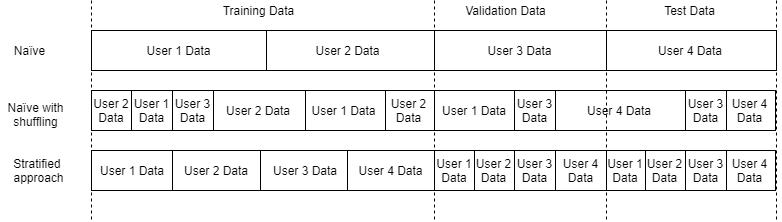
\includegraphics[width=\linewidth]{resources/split.png}
	\caption{A visual representation of the data splitting approaches.}
	\label{fig:split}
\end{figure}
\noindent Algorithm~\ref{algo:strat_collection} illustrates the stratified split idea well by using pseudocode. For every user, the data is split and added to a collection of the same type of data. After iterating through all the users, the collections are used to set the train, test and validation data for the $global\_user$.
\begin{center}\begin{algorithm}[H]
\Fn{\FDataSplit{users}}{
	unioned\_train = [ ]\\
	unioned\_validation = [ ]\\
	unioned\_test = [ ]\\
    \For{\forcond{$U_i$}{$users$}}{
	    train, validation, test = split\_user\_data($U_i$)\\
	    unioned\_train.append(train)\\
	    unioned\_validation.append(validation)\\
	    unioned\_test.append(test)\\
    }
    global\_user = User()\\
    global\_user.set\_train\_data(unioned\_train)\\
    global\_user.set\_validation\_data(unioned\_validation)\\
    global\_user.set\_test\_data(unioned\_test)\\
    \textbf{return} global\_user
  \caption{Stratified data collection for the global user}\label{algo:strat_collection}
}
\end{algorithm}\end{center}
\noindent To initialise the $global\_user$, a model also needs to be found that works of the given dataset. Naturally, this process is specific to the dataset being used and will be covered in more detail sections where we talk about specific datasets. The process of finding an $M$ that fits the dataset well is an empirical one. It involves numerous experiments with different model architectures and tweaking of hyper-parameters. The model with the best metrics on the validation data is selected as $M$. The important thing to note here is that the model that the $global\_user$ ends up using is the model that every user in the federated learning process will use as well. This is done because if a model that performs well in a non-federated context is used in the federated context as well, questions about selecting models that specifically work well in a federated learning environment are not raised. 
\\\\
For the \texttt{implementation} of the splitting, we start by reading the dataset into Python. Reading in the dataset is specific to the dataset being used, based on whether a csv file is provided or a directory structure is being traversed to acquire the data. This, the preprocessing and the allocation of data to the users is discussed further in the sections where we talk about specific datasets. The number of users $n$ is also, depending on the dataset, decided or found here. For now, we assume that every user object has the data belonging to it and only the splitting is required.
\\\\
To handle the splitting of data into the three parts, we implement context specific functions that would be used based on the type of input dataset being used which can be either based on a DataFrame or numpy arrays. We can call them \texttt{split\_dataframe} and \texttt{split\_numpy}. The parameters for these functions include \texttt{dataset}, \texttt{for\_user}, \texttt{val\_size}, \texttt{test\_size} and \texttt{seed}. The values for \texttt{test\_size} and \texttt{val\_size} in this project were 0.2 and 0.2 respectively, giving 0.6 to the training set. These fractions represent the fraction of the input dataset to be allocated to the three named subsets. The logic of the splitting requires the input data to first be split into training and test data on the specified split ratios of 0.8 and 0.2 respectively. In \texttt{split\_numpy}, where we deal directly with numpy arrays, for the splitting we use the \texttt{split} function provided by numpy to split an array based on the given ratio. In \texttt{split\_dataframe}, where the splitting is done on DataFrames, we use scikit-learn's \texttt{train\_test\_split} function to split the DataFrame based on the given ratio. To ensure reproducibility, we use a \texttt{seed} for every randomised operation used in this project. The \texttt{train\_test\_split} function uses this as it shuffles the input DataFrame before splitting it. Then the training data must be split into training and validation data. As the split now takes place on 80\% of the input data, we need to adjust \texttt{val\_size} to ensure that the correct split ratios are maintained with respect to the full input data size. To do so, \texttt{val\_size} needs to be recalculated as in equation~\ref{eq:val_size}. 
\begin{equation}\label{eq:val_size}
	val\_size = \frac{val\_size}{1-test\_size}
\end{equation}
The training set is then split into training and validation data based on the new \texttt{val\_size} using the same methods, depending on the function that calls them. This data is stored in User objects for every user with the data being stored as features and labels separately. 
\\\\
To get the three parts of data for the global user in a stratified manner, we iterate over all the user objects $U_i$ and call one of the above functions on them to split their dataset into the three parts. After every user has been assigned their training, testing and validation data, we iterate over them once more to allocate data to the $global\_user$. For every user object $U_i$, we get each of the three parts and add them to the respective parts in the $global\_user$ by using the appropriate object method. These methods can be see in Figure~\ref{fig:classes_user}. For instance, for every user object $U_i$ we get their test data and it's label using the \texttt{get\_test\_data} and \texttt{get\_test\_class} and add it to the $global\_user$ object using the \texttt{add\_test\_data} and \texttt{add\_test\_class} methods respectively. This, when done for all three parts and all users, results in a stratified collection of data for the $global\_user$ with respect to individual user data.
\\\\
We did not use the stratified idea with regards to the classes as we thought it would not be realistic to do so. The reason behind this was that the user might have data that is coming in on the fly, and to be splitting it based on classes means that the classes of the incoming data is already know. This would not be true in a real world scenario. To uphold that idea, we did not use the stratified idea on the classes when making the splits.
\\\\
We have to then try to find a model $M$ that performs well on the dataset. Keras provides an API to construct a model with relative ease. It allows us to construct a layer of neurons and stack them on top of each other to build an architecture suitable for our needs. The models we create are sequential feed forward models that use the \texttt{Sequential} object. We can layers of neurons to this object by using the \texttt{add} method of the object or we can initiliase the object with a list of constructed layers. The layers are created using the appropriate method to initialise the kind of layer being used. They include, but are not limited to, the layers mentioned in Section~\ref{subsec:arch}. To create a dense layer, a \texttt{Dense} object is created with the parameters being the number of nodes in the layer and the input shape. For a 2D convolutional layer, a \texttt{Conv2D} object is created with the feature map count and window size as the parameters. The use of the layers is dataset specific. When we create the layers, we also pass in the activation functions for the layers. These were always the ReLU activation function in this project for all the hidden layers, and for the output layer it was always softmax. This is because the experiments were conducted only of classification problems. The functions were passed in as string names like \texttt{relu} and \texttt{softmax} for the \texttt{activation} parameter when constructing the layers. Their common usage meant that Keras has those functions built into their framework and we can access them using just the strings. We also initialised all the starting weights of the models randomly using a standard seed. The \texttt{keras\_initializer} parameter during the construction of the layer was provided with the \texttt{keras.initializers.glorot\_uniform} function with a seed. This would initialise every weights vector in the model with the same weights every single time. The usage of a seed to initialise the weights results in every user having the exact same model. It also gives us reproducible results when the training is performed on the CPU. When training is performed on a GPU, the parallelised nature of the operations meant that the results were not reproducible. This was a limitation of using Keras, as there are other options with lower level controls that allow us to seed the parallelised operations that take place in the GPU itself. But without that, we cannot guarantee fully reproducible results.  
\\\\
After constructing the architecture, Keras requires for the model to be compiled. To do so, the \texttt{compile} method is called on the model that we just created. This method takes in \texttt{optimizer}, \texttt{loss} and \texttt{metrics} as its parameters. The optimizer is used during the training process by Keras and we specify Keras to use the \texttt{adam} optimiser. This is the an optimizer that is said to work well for most cases, and for both of our datasets it seemed to perform pretty well. Hence it was chosen as the standard. The loss is used during the training process to know how far the predictions are from the truth. We chose \texttt{sparse\_categorical\_crossentropy} as the loss throughout out project as it empirically gave the best results from the other loss methods we had tried. Also, for a classification problem, this seems to be the go-to loss function. The optimizer and loss as passed in as strings to the parameters. The metrics parameter takes in a list of metrics that are to be evaluated by Keras itself in the training process. These are stored in the history object in the Keras model. We chose \texttt{SparceCategoricalAccuracy} as the metric to measure in the training process as it is the standard choice to take when using the aforementioned loss function. For all the models we use in this project, the same parameters were used for the compilation process. They were all empirically found to be the best option for both the datasets. 
\\\\
To find the best model $M$, several different architectures are tested on the dataset in question. The tests included training the model on the training data and then plotting a graph of evaluations versus epochs to see how the model progresses over time. The metric of choice was always accuracy. The plots were made for both, the performance of the model on the training data and the validation data. Efforts were made to ensure that the model was not suffering from over-fitting or under-fitting. The plots were very useful in checking for that. An indication of over-fitting is that the metrics of the validation data and training data begin to diverge. In this case, the model is made a bit simpler. Techniques include reducing the number of neurons, number of layers, adding regularization or adding a dropout layer (where certain neuron outputs are ignored). A sign of under-fitting is that the metrics are too ``bad", for instance the accuracy being too low. In this case, we can do the opposite of what we do in the case of over-fitting. All of these techniques can be easily implemented in Keras using the API it provides to create and edit layers. 
\subsubsection{Federated Users}
The initialisation of the federated users shares components with that of the global user. The logic about splitting a specific user's data into training, testing and validation data applies here as well. We assume that the user knows what its local data is, more detains about this can be seen in the sections relating to specific datasets. This data is split into the three parts as explained in the previous section. The model found for the global user is used by the federated users for their local learning as well to make the experiment fair. To do so, the model $M$ that the was found for the global user is simply given to every user during the initialisation process.
\\\\
The design for splitting data for every user is exactly the same as that of the global user. In the global user, there is another step after splitting the data which is to union the data from every user. This step is not required for the federated users. Because the design is the same, the \texttt{implementation} is exactly the same as well. We iterate over all the users and call the appropriate function, depending on the type of data being dealt with, to split the user's data into the three parts. These are stored as the data and the label for every part in attributes of the user object as multi-dimensional numpy arrays. The additional step of passing in the model is done by encapsulating the creation and compilation of the model into a function called \texttt{init\_model}. This constructs and compiles a model, for a given dataset, and returns a compiled Keras model object. This function is called for every user such that every user gets an identical copy of the model and they store as an attribute in the user object that represents them. 
\subsection{Graphing}
In this section we will describe the graphs that are generated for the experiments we conduct. We used line graphs in this project as it made the most sense to use them to plot the progress of the average evaluations for all users over the rounds. The line of the average also had regions above and below it, indicating certain information. This information could be one of two options that we chose to display. The first option is to have a region covered by the minimum and maximum values of the user for every round. We call this the $min\_mix\_fill$. The second option is where the region covers an area of one standard deviation away form the average of the user for a round. We call this the $std\_dev\_fill$. The idea of this filled in region made the graph look like a sausage, and hence we coined the term ``sausage graphs'' for this idea. The evaluations of both the $pre\_fit$ and $post\_fit$ were both plotted on the same graph with colour coding. A lighter shade of the colour was used to fill in the regions. An example of this can be seen in figure~\ref{sample_graph}.
\begin{figure}[H]
	\centering
	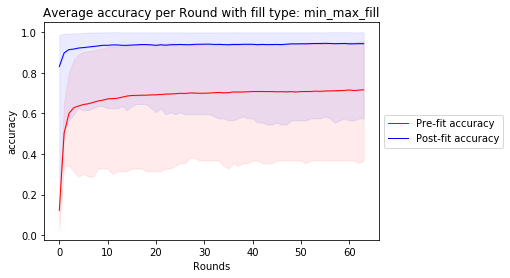
\includegraphics[width=10cm]{resources/sample_graph.png}
	\caption{An example to show the sausage graph idea.}
	\label{fig:sample_graph}
\end{figure}
\noindent The same idea was used to plot a graph where the users were on the x-axis instead of the rounds, but after implementing it we realised it does not give any useful information about the process. So we decided to abandon the graphs made from that idea. The design for both of them is largely similar, so we will discuss only the more useful plotting method where we plot the evaluations versus rounds graph. 
\\\\
When designing this, the simplified idea was to get the data from all the users, process it to get the statistics we need and then plot it. To do so, we first iterate over all the users and get the statistics that we need from their evaluations to plot the graph. This includes information like the number of rounds, average, standard deviation, minimum evaluation and maximum evaluation. After getting the information we need we can simply go ahead and plot the average line and then use the statistics we gathered to fill in the area depending on the fill type being used. This done for both $pre\_fit$ and $post\_fit$ evaluations and the final graph is then ready. 
\\\\
The \texttt{implementation} was quite time consuming in terms of implementing it in a way that made the code reusable. Since we only use the graphs of evaluation vs rounds, we will only talk about its implementation in-depth. But the evaluations versus users graph is very similar, it is just plotted in a different way. We start off by getting the users data. The function responsible for getting this data is provided with the dictionary of users for a given idea, $U_{idea}$. Then we iterate over the users in that dictionary and use the \texttt{get\_data} method on the user object which returns the $post\_fit$ or the $pre\_fit$ evaluations as numpy arrays based on the functions parameters. These are collected in another numpy array to create a multi-dimensional array. Using this data we get the statistics that we will be using. By using the number of evaluations a user has, we get the number of rounds. The average, standard deviation, minimum and maximum evaluations can be acquired by calling the \texttt{average}, \texttt{std}, \texttt{amin} and \texttt{amax} respectively on the 0th axis on the numpy array that contains every users evaluations. This will result in us getting the round-wise statistics calculated from the evaluations of every user. This is done for both $pre\_fit$ and $post\_fit$ evaluations to get the statistics for each. These statistics are then labelled and organised into a pandas DataFrame for ease of use which we call $df_{idea, round}$. We then use this DataFrame for the plotting process.
\\\\
We use pyplot from the matplotlib library, which we call \texttt{plt}, for plotting the graphs. The column in $df_{idea, round}$ containing the averages of all users for every round is used to plot the main line. To do so, we provide to the \texttt{plot} method of \texttt{plt} a list of number of the rounds for the x-axis and averages of both $pre\_fit$ and $post\_fit$ evaluations individually for the y-axis to be able to plot the two lines. They are colour coded with $pre\_fit$ being red and $post\_fit$ being blue. We then fill the region around the main line based on the filling strategy. To do so, we use the \texttt{fill\_between} method of \texttt{plt}. This method takes in a list of numbers representing the rounds for the x-axis and takes in two parameters as arrays for the limits of the fill region. For these, based on the filling strategy, we pass in different data. For the $std\_dev\_fill$, we provide $average\_array + standard\_deviation\_array$ as the upper limit and $average\_array - standard\_deviation\_array$ as the lower limit. For the $min\_mix\_fill$ we, call the \texttt{fill\_between} twice. The first time we give the array of minimum evaluations for the lower limit and the array of averages as the upper limit. For the second call, we provide the array of averages as the lower limit and the array of maximum evaluations for the upper limit. An alpha value of $0.08$ is used to colour the regions as a lighter shade of the main colour. The method then fills the region based on the upper and lower limit using the specific colour and alpha value that we chose. After both the lines and their regions have been plotted, we are finished with the plotting process and return the $df_{idea, round}$ DataFrame for usage in collecting the summary report as previously described. The graphs are also saved to disk using the \texttt{savefig} method. Figure~\ref{fig:sample_graph} is a sample of the evaluations versus rounds graph with the $min\_max\_fill$ filling strategy. 
\\\\
The same basic process, with a few changes, is followed for the evaluations versus users graph. The process is also still done for both $pre\_fit$ and $post\_fit$ evaluations. The user IDs are now used for the x-axis instead of the rounds. The statistics are calculated from the evaluations over the rounds for a user instead of over the users for a round. They are now user specific statistics and not round specific statistics. The same methods allow us to get them, but we call the methods on individual user's collection of evaluations instead of the evaluations of all users for a given round. The final evaluation value is also return as part of the statistics. These statistics and compiled into a DataFrame which is used for the plotting process as described above. The final values are organised into a separate DataFrame which is returned as $df_{idea, user}$ for use in collecting the summary report later. For the global user who performs non-federated learning, we only plot the line of evaluations obtained from the history object of the Keras model. 
\subsection{Postures Dataset}\label{subsec:gestureset}
In this and the following section, we will talk about the experiments conducted on specific datasets. This particular dataset, named ``MoCap Hand Postures Data Set'', was acquired from the UCI Machine Learning Repository~\cite{Dua:2019} as a csv file. It was the first dataset we used to conduct experiments. It is a dataset where a Vicon motion capture camera system was used to record data about 12 users performing 5 hand postures using their left hand. The data that we get are coordinates from a glove, with markers on it, that was worn on the left hand of the user.  
\\\\
The markers were broken down into two sets. The first set of markers was on placed the back of the glove in a rigid patter and was used to establish the local coordinate system for the hand. The second set was attached to the thumb and the fingers. This second set of markers were not labelled, so their positions were not explicitly tracked. This meant that there was no relation between the markers of two given records. Due to the resolution of the capture volume and self-occlusion due to the orientation and configuration of the hand and fingers, a lot of the records have missing marker values. Due to the manner in which the data was captured, there was also a chance that there was a near duplicate record that originated from the same user. The fact that two records could not be directly compared and a lot of marker values were missing made this quite an awkward dataset to work on, but we still gave it a shot to see how it worked with our ideas. The 
\\\\
Some preprocessing was performed on the dataset by the providers before sharing it. This included removing records with less than three marker values and transforming the coordinates to the local coordinate system of the record containing them. We assumed that this also takes care of scaling the data to the scale of the local coordinate system. The dataset came with columns for the x, y and z coordinates for all the markers, a column to label the hand posture and a column to label the user the data belongs to. The labels for the hand postures were enumerated as numbers.
\subsubsection{Data separation}
All the ideas about federated learning we have seen in this project assumed that every user knew what data belonged to them. In the section about user initialisations, we once again assumed that the user knows what data belongs to them. But in an experiment, that is not the case. The data needs to be separated by allocating to the users the data that belongs to them. The process for doing so in this dataset was very simple. The dataset came with a column ``UserID'' which labelled every record with the user ID of the user that the record was from. 
\\\\
The idea is to read in the csv file and impute the missing values with zeros. Then iterate over records in the csv file and based on the ``UserID'' column, separate the data to allocate them to the simulated user representations. 
\\\\
To \textit{implement} this, the csv file is read into a pandas DataFrame using the \texttt{read\_csv} method provided by the pandas library. We call this DataFrame $df$. Before doing any work on the separation, we need to impute the missing values in the records. They were noted down as ``?'' which we then replaced with zeros. To do so, we first use the \texttt{replace} method on $df$ to replace the ``?'' with a special numpy value called \texttt{nan}. These \texttt{nan}'s are then replaced by zeros using the \texttt{fillna} method on $df$. We can can then move on to allocating data to the users to the point where the we can split them into training, testing and validation data before starting the training process.
\\\\
As the ``UserID'' column indicates what user a record belong to, filtering the $df$ on the user ID column is enough to separate the data. Pandas DataFrames have a filter functionality that allows us to do this with ease. First, we find the unique user IDs in the column which we can easily do by calling the \texttt{nunique} method on the $df$. We then iterate over all the user IDs and filter $df$ based on the user ID $i$ so it returns a DataFrame that contain data only for a particular user $U_i$. The DataFrame containing data for user $i$ is called $df_i$. This $df_i$ is then split into training, testing and validation data for the user and resulting partitions stored in a User object. The same process is done for every federated user represented by the user IDs so we have User objects initialised with the three part data. 
%\begin{center}\begin{algorithm}[H]
%\Fn{\FDataSepCsv{df}}{
%	\# returns a list of unique user IDs\\
%	user\_ids = df["UserID"].unique() \\
%	\For{\forcond{$user_id$}{$user_ids$}}{
%		\# returns a DataFrame with data for user with ID $user_id$\\
%	    df\_user = df[df["UserID"] == user\_id]\\
%	    
%		user\_dfs.append(df\_user)
%    }
%  \caption{Data separation for csv files with user IDs}\label{algo:dataset-csv}
%}
%\end{algorithm}\end{center}
\subsubsection{Model Selection}
To select the model for this dataset, we first initialised the global user and then trained several models on it to see which one performed relatively well. Because of the fact that two records could not be compared directly, we thought a convolutional neural network was not the ideal choice for this dataset. So we chose to build a dense network. The goal is to have a model that is simple and performs well. There is no point in making a more powerful model if the performance does not increase significantly from it as more powerful models take way longer to train. So we started off with a deep network and started tweaking its size and node count to a point where the performance was essentially the same as the deeper models but with a significant reduction in the parameter count. The architecture shown in Figure~\ref{fig:posture_model}, with three dense with node counts of 512, 128, 32 and 5 was chosen as the final model $M$ that was to be used by the global user and all the federated users. 
\begin{figure}[H]
	\centering
	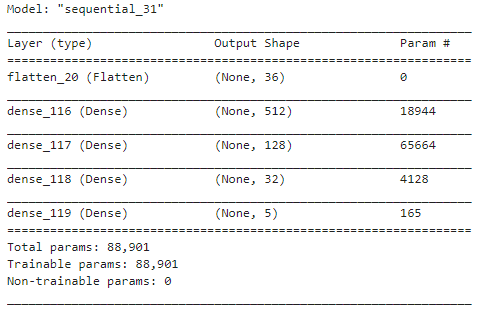
\includegraphics[width=10cm]{resources/posture_model.png}
	\caption{Architecture of the model used for the postures dataset.}
	\label{fig:posture_model}
\end{figure}
\noindent We use Keras to build the models, starting off with a flatten layer that flattens the data into a 1D numpy array. The subsequent layers are made with \texttt{Dense} layer objects with node counts of 512, 128, 32 and 5. The final layer is the \texttt{Dense} layer with five nodes in it and they represent the five postures in this dataset. The initial weights of the model are seeded as mentioned before. The compiled version of this architecture is used by the global user and federated users. We store a copy of this model in every user's User object for them to use locally.
\subsubsection{Results}
With the data and the model ready, we run the experiments and record the results as explained in Section~\ref{subsec:framework}. The experiments were ran where 64 rounds of federated learning took place with the local epoch count being 16. For the global user, the experiment ran for $64 \times 16$ epochs.
\\\\
\begin{figure}[H]
\centering
\begin{subfigure}{0.45\textwidth}
    \centering
    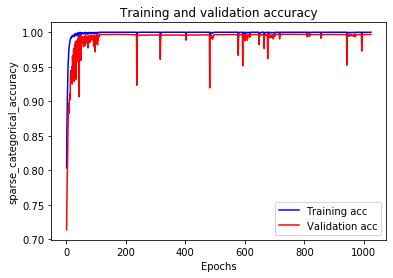
\includegraphics[width=\textwidth]{resources/posture_global_stdsplit-accuracy.png}
    \caption{Global user}
    \label{fig:posture_graphs:global}
\end{subfigure}%
\\
\begin{subfigure}{0.45\textwidth}
    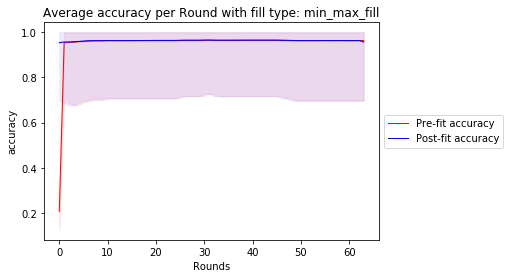
\includegraphics[width=\textwidth]{resources/posture_localround-stdsplit-accuracy.png}
    \raggedleft
    \caption{Local Training}
    \label{fig:posture_graphs:local}
\end{subfigure}
\begin{subfigure}{0.45\textwidth}
    \raggedleft
    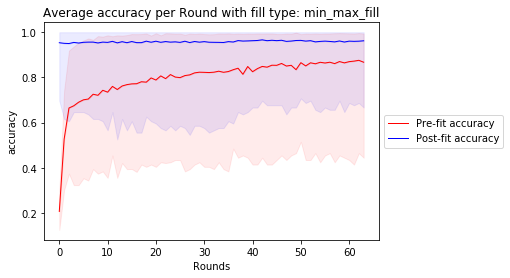
\includegraphics[width=\textwidth]{resources/posture_centralround-stdsplit-accuracy.png}
    \caption{Central Standard Averaging}
\end{subfigure}%
\\
\begin{subfigure}{0.45\textwidth}
    \raggedleft
    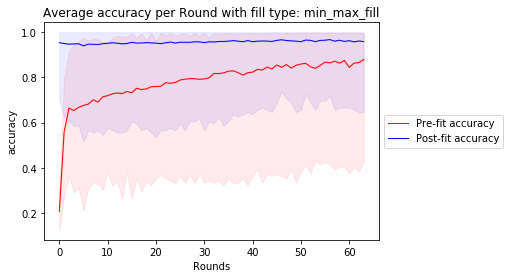
\includegraphics[width=\textwidth]{resources/posture_stdround-stdsplit-accuracy.png}
    \caption{Central Selective Inclusion}
\end{subfigure}
\begin{subfigure}{0.45\textwidth}
    \raggedleft
    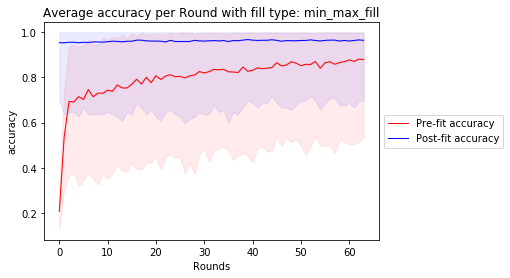
\includegraphics[width=\textwidth]{resources/posture_stdround_p2p-stdsplit-accuracy.png}
    \caption{Peer-to-peer Selective Inclusion}
\end{subfigure}
\\
\begin{subfigure}{0.45\textwidth}
    \raggedleft
    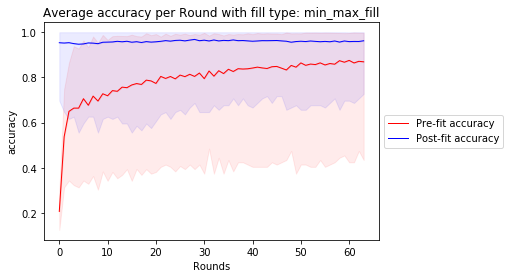
\includegraphics[width=\textwidth]{resources/posture_weightround-stdsplit-accuracy.png}
    \caption{Central Weighed Averaging}
\end{subfigure}
\begin{subfigure}{0.45\textwidth}
    \raggedleft
    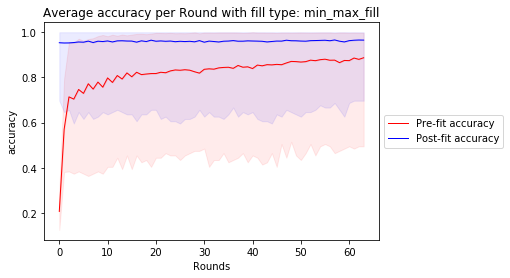
\includegraphics[width=\textwidth]{resources/posture_weightround_p2p-stdsplit-accuracy.png}
    \caption{Peer-to-peer Weighed Averaging}
\end{subfigure}
\caption{Graphs for the experiments on the postures dataset.}
\label{fig:posture_graphs}
\end{figure}
\noindent The graphs in Figure~\ref{fig:posture_graphs} show the progression of the ideas in a round-by-round manner with the $min\_max\_fill$ fill style which shades the region between the highest and the lowest evaluations. On the x-axis we have the rounds, except for Figure~\ref{fig:posture_graphs:global} where the x-axis is epochs, and on the y-axis we have the evaluations for which we used accuracy as the metric. For all the graphs, bar Figure~\ref{fig:posture_graphs:global}, the evaluations are averages of every users evaluations on their local testing data in the $pre\_fit$ and $post\_fit$ context. 
\\\\
The global user's graph shows its learning curve, where the lines are based on evaluations made on the training data and the validation data. Naturally, the global user's evaluations will be higher because it has access to a wider range of data. We do not use its graph as a benchmark because it shows the evaluations obtained on data that is not the testing data, whereas for the other graphs the evaluations were made on local testing data. For all the other ideas we implemented, we can see that they are all performing pretty close to one another except Figure~\ref{fig:posture_graphs:local} which shows the progression of the local training idea. This idea shows an average of pretty much 100\% as the user only gets exposure to its own data and gets very good at predicting it. But this is not necessarily good news as the users do not get exposure to the knowledge that the other users posses. Which means that even though the models are good at predicting data specific to a user, they might not be able to perform so well when a wider variety of data is presented to them. The benefits depend on the context but in the general case it is better to have learnt generic characteristics from a wide range of samples instead of user specific characteristics. The general trend seen in the other graphs is that the $post\_fit$ line is always very high, which makes sense as after training the model on the local training data its evaluations on the local testing data would be good. The $pre\_fit$ line, which plots evaluations made on the averaged weights, shows improvement as the rounds progress. This means that the federated learning process is gaining more knowledge from all the users in every round. 
\\\\
The graphs also show a peculiar characteristic of the peer-to-peer ideas. We can see that thier lowest evaluations (as seen from the lower line in light red filling) are higher than the lowest evaluations seen in their central averaging counterparts. This is probably because the users average the weights based on what is good for them personally and by doing so their local evaluations are better than the ones with the central averaging approach. Other than this, all the graphs, bar the local training graph, seem to show pretty similar performance between all the ideas, including the standard idea.
\begin{table}[H] % prefit -----------------------------------------------------------
\def\arraystretch{1.2}%
\resizebox{\linewidth}{!}{\begin{tabular}{|c|c|c|c|c|c|c|} %lllll
\hline
& \makecell{Local\\Training} & \makecell{Central\\Standard\\Averaging} & \makecell{Central\\Selective\\Inclusion} & \makecell{P2P\\Selective\\Inclusion} & \makecell{Central\\Weighted\\Averaging} & \makecell{P2P\\Weighted\\Averaging}\\
\hline
Average & 96.34\% & 86.73\% & 87.89\% & 87.95\% & 86.91\% & 88.71\%\\
\hline
\makecell{Standard\\Deviation} & 8.27 & 16.96 & 17.71 & 14.56 & 17.09 & 14.95\\
\hline
Lowest & 69.70\% & 44.44\% & 42.42\% & 53.54\% & 43.43\% & 49.49\%\\
\hline
Highest & 100.00\% & 99.43\% & 99.60\% & 99.83\% & 99.77\% & 99.77\%\\
\hline
\end{tabular}}
\caption{Posture dataset: Pre fit results at the end of the rounds from testing user models.} \label{tab:postures_pre_fit}
\end{table}

\begin{table}[H] % postfit -----------------------------------------------------------

\def\arraystretch{1.2}%
\resizebox{\linewidth}{!}{\begin{tabular}{|c|c|c|c|c|c|c|} %lllll
\hline
& \makecell{Local\\Training} & \makecell{Central\\Standard\\Averaging} & \makecell{Central\\Selective\\Inclusion} & \makecell{P2P\\Selective\\Inclusion} & \makecell{Central\\Weighted\\Averaging} & \makecell{P2P\\Weighted\\Averaging}\\
\hline
Average & 95.70\% & 96.23\% & 95.90\% & 96.43\% & 96.24\% & 96.52\%\\
\hline
\makecell{Standard\\Deviation} & 8.32 & 9.07 & 9.78 & 8.30 & 8.11 & 8.20\\
\hline
Lowest & 69.70\% & 66.67\% & 64.65\% & 69.70\% & 72.73\% & 69.70\%\\
\hline
Highest & 100.00\% & 100.00\% & 100.00\% & 100.00\% & 100.00\% & 100.00\%\\
\hline

\end{tabular}}
\caption{Posture dataset: Post fit results at the end of the rounds from testing user models.} \label{tab:postures_post_fit}
\end{table}
\noindent To get a better idea of the performance, we look at the statistics from the final $pre\_fit$ and $post\_fit$ evaluations of the ideas in tables~\ref{tab:postures_pre_fit} and~\ref{tab:postures_post_fit}. We can see that the highest evaluations in either set of evaluations are very close to 100\%, if not 100\%. This means that some users are probably benefiting a lot from the federated learning process. But we can also observe from the lowest evaluations that some are struggling. This could be due to the fact that in this dataset, records cannot be directly compared and the weights from models learnt on different datasets could cause hindrances in the training process for certain users, for example the ones that are not performing well. Our hypothesis regarding the peer-to-peer ideas is also solidified here as we can see that in most cases, the peer-to-peer ideas have a higher value in the ``Lowest" evaluation section when compared to their central averaging counterpart. Their standard deviations are also lower. And the averaging process is still anonymous as the users do not know the owner of the weights, so we can say that the peer-to-peer idea seems to be provided a better overall approach with better metrics than the central averaging counterparts whilst maintaining privacy. The general trend of the metrics being better in the $post\_fit$ evaluations compared to the $pre\_fit$ evaluations is because the users train their model on their local data and then evaluate it once again on their local test data. Expectedly, this training process makes them better at recognising the patterns in their local data which results in their metrics getting better. 
\\\\
Table~\ref{tab:postures_on_global_user} reiterates the fact that the local training idea was the best performing one for a given user in terms of the evaluations done on the local testing data. No other federated idea could come close to it in the $pre\_fit$ evaluation where the evaluations on the freshly averaged weights are compared. But this is because the $pre\_fit$ evaluations are essentially redundant in this case and not weight sharing process takes place. So we look at the $post\_fit$ performance where all the users were performing better than the local training idea and would probably perform better than it when met with a wider variety of unseen data as well. This is once again because the local training idea only focusses on the user's dataset and does not avail of the knowledge learnt by other users. It is pretty safe to say that the metrics from the local training approach are misleading as we will find out in the following section.
%\subsubsection{Testing on global user}
\\\\
The evaluations seen earlier were conducted on every user's local testing data. We wanted to see how their local models would fare on a more generic dataset that contained data from every user. So we decided to evaluate every user's model on the global user's testing data. The global user's test data contains about 20\% of every user's data. Here we also evaluated the global user, which uses the non-federated approach, for the first time on its test data. The results are seen in Table~\ref{tab:postures_on_global_user}.
\begin{table}[H]
\def\arraystretch{1.2}%
\resizebox{\linewidth}{!}{\begin{tabular}{|c|c|c|c|c|c|c|c|} %lllll
\hline
 & \makecell{Non\\Federated} & \makecell{Local\\Training} & \makecell{Central\\Standard\\Averaging} & \makecell{Central\\Selective\\Inclusion} & \makecell{P2P\\Selective\\Inclusion} & \makecell{Central\\Weighted\\Averaging} & \makecell{P2P\\Weighted\\Averaging}\\
 \hline
User 0 &  & 61.08\% & 75.22\% & 73.82\% & 78.78\% & 78.47\% & 82.09\%\\
\hline
User 1 &  & 56.92\% & 76.78\% & 73.43\% & 75.70\% & 67.98\% & 70.26\%\\
\hline
User 2 &  & 49.99\% & 57.58\% & 71.96\% & 64.77\% & 60.17\% & 63.99\%\\
\hline
User 4 &  & 40.73\% & 59.42\% & 59.69\% & 54.57\% & 59.99\% & 61.59\%\\
\hline
User 5 &  & 48.35\% & 75.63\% & 77.86\% & 78.31\% & 75.58\% & 76.35\%\\
\hline
User 6 &  & 63.07\% & 84.57\% & 82.75\% & 87.47\% & 85.57\% & 71.20\%\\
\hline
User 7 &  & 49.43\% & 82.56\% & 75.92\% & 83.41\% & 82.92\% & 83.68\%\\
\hline
User 8 &  & 54.42\% & 75.17\% & 72.93\% & 71.72\% & 71.06\% & 65.71\%\\
\hline
User 9 &  & 61.96\% & 78.72\% & 84.15\% & 85.26\% & 84.98\% & 83.41\%\\
\hline
User 10 &  & 53.25\% & 86.94\% & 85.92\% & 75.03\% & 79.30\% & 74.57\%\\
\hline
User 11 &  & 59.82\% & 81.58\% & 78.52\% & 73.41\% & 78.79\% & 69.38\%\\
\hline
User 12 &  & 56.66\% & 89.94\% & 89.90\% & 89.98\% & 90.66\% & 88.27\%\\
\hline
User 13 &  & 59.86\% & 88.41\% & 90.49\% & 86.56\% & 87.34\% & 82.58\%\\
\hline
Average & 99.64\% & 55.04\% & 77.88\% & 78.26\% & 77.30\% & 77.14\% & 74.85\%\\
\hline
\end{tabular}}
\caption{Posture dataset: Results from testing user models on global user's data.} \label{tab:postures_on_global_user}
\end{table}
\noindent The table shows the evaluation of every user's models from every idea on the global user's testing data. Their averages show numbers that we can use to compare how good the models created by those ideas were on generic testing data. It is evident that the averages for every idea are lower than that when the evaluations were done on the user's local testing data because now the testing set is more varied. We can see, as expected, the local training idea does not fare well here at all because of the lack of shared knowledge gained from federated learning. All the other ideas beat this benchmark, but cannot come close to the non-federated approach which has a very high accuracy. 
\\\\
The other ideas, for the most part, are very close to one another though, implying that they did not have that big of an impact on the training process. But because of that, we can also say that we can get better privacy using our peer-to-peer ideas with minimal performance loss. This is because a peer-to-peer approach decentralises the process and removes all doubt that the central agent could learn anything from any user's weights. It also means that the calculations of the averaging and re-evaluations take place on the edge device, which means it takes more resources on the edge device. This is a trade-off that must be decided on, a little bit more privacy for more processing to be done on the edge device. The peer-to-peer idea is also probably a bit better for individual users because of its higher values in the lowest evaluations section, which means that individual users benefit more whilst maintaining the idea of shared knowledge which benefits them overall when exposed to more varied data. This hypothesis is backed up by the results we can see in Figure~\ref{fig:posture_graphs} and Tables~\ref{tab:postures_pre_fit} and~\ref{tab:postures_post_fit}.
\subsubsection{Sanity check using TFF}
Section~\ref{subsec:tff} explained how TFF can be used to conduct federated learning once the dataset is separated based on the users and placed in Dataset objects that TFF can use for its learning process. We will now look at the process of placing the data in Dataset objects for TFF to perform federated learning and we will compare the evaluation results with our implementation of standard federated learning for a sanity check. 
\\\\
Converting an arbitrary dataset into a Dataset object is not well documented by TFF's documentation yet, so the process of implementing this consisted of a lot of trial and error. We found that TFF provides a way to read HDF5 (Hierarchical Data Format version 5) files into client data in the form of Dataset objects. We can do so by instantiating the \texttt{hdf5\_client\_data.HDF5ClientData} class with the path of the HDF5 file as the parameter and this returns a Dataset object that TFF can use for the training.
\\\\
So we had to find a way to split and convert our dataset into two HDF5 files, one for training and the other for testing in an 80-20 split. To do this, we read the csv dataset into a DataFrame using the \texttt{read\_csv} function and split it into the two parts using the \texttt{train\_test\_split} function with a ratio of 80-20 for training to testing data. This is done using a stratified idea, where the training DataFrame contains 80\% of every user's data and the testing DataFrame contains 20\% of every user's data. 
\\\\
Each DataFrame is then used to create a HDF5 file. HDF5 is a file format that allows us to store data in a ``file directory" like structure. The h5py library allows us to create HDF5 files in Python. The structure required for the files is as such, the top top level group is called ``examples" and inside it, for every user, there is a group labelled with the user ID. The groups are created using the \texttt{create\_group} function on the h5py \texttt{File} which is the file we are using and writing to disk. Inside the group, for every user $U_i$, we use the \texttt{create\_dataset} function to create datasets labelled $points$ and $label$ containing the features and the classes of the samples respectively. We get this data by filtering the DataFrame to get user specific data and then separate the features and the classes from it by using the DataFrame API. After every user's data is stored in this structure in both HDF5 files, we can provide the path to these files to the \texttt{hdf5\_client\_data.HDF5ClientData} class so we can get the Dataset objects that we need.
\\\\
We then use the \texttt{create\_tf\_dataset\_for\_clients} method on the Dataset objects to create the training and testing data that TFF can use for training and evaluation. This has to be done for every user and a list of them is returned as the training and testing data. The dataset, after creation, is preprocessed to indicate the batch size and epochs that could be used in the training process. The features are also flattened and mapped to their class label in an ordered dictionary. This, when done for both training and testing data, provides us with the data that the TFF can use in its learning process as described in Section~\ref{subsec:tff}.
\\\\
After everything was ready, we ran the TFF learning process for 16 rounds, 16 epochs and the batch size being 20 and got an accuracy of $79.47\%$. We then ran our implementation of federated learning as well using the same parameters and got an accuracy of $76.18\%$. There was only a difference of about $3\%$ and because the difference was so small, we got confidence that our implementation of federated learning was logically correct and hence the sanity check was successful. 
\\\\
We then chose to move onto a different dataset because this dataset had some drawbacks that made it awkward to work with. For instance, the records could not be compared with each other directly and that several marker values that were missing from the records. We also wanted to see how the ideas we implemented in this project would fare on a different dataset with a more complicated model.
\subsection{Image dataset}\label{subsec:imageset}
So for out next dataset, we chose an image based dataset named ``Natural Images''~\cite{roy2018effects} which was acquired from Kaggle as a set of 6,899 images of eight classes. The classes of images are airplane, car, cat, dog, flower, fruit, motorbike and person with no less than 700 images per class. The images were placed in directories that were named according to the class the image belongs to. The dataset was not user focused and was therefore not labelled with what image belong to what user.
\subsubsection{Data Separation}
As the data was not user focussed, we had the creative license to separate the data in a method of our choice. We chose an approach where we would have the same number of users as there are classes of images, eight. Every user $U_i$ would be ``in-charge'' of a class $C_i$ such that certain portion of $C_i$ is allocated to $U_i$ and the remaining images of $C_i$ are distributed amongst the other users. The amount of $C_i$ that $U_i$ gets is based on a probability $P$. By doing this, we are simulating a federated dataset. After this is done, the data is split into the training, testing and validation data for every user.
\\\\
To separate the data and allocate them to users, we have to iterate over all the image classes $C$. For every image $I_{C_i, j}$ in class $C_i$, user $U_i$ has a probability $P$ of acquiring $I_{C_i, j}$ for its local dataset. The images of $C_i$ that $U_i$ does not acquire are then split amongst the other users with equal probability. This is done for every image class and at the end, every user has a local dataset that has been distributed in a probabilistic manner. 
\\\\
To \texttt{implement} this, we need to first create a mapping of all the classes to their respective images. We use a dictionary, called $image\_mapping$, to create a mapping of all the classes of images to a list of numpy arrays of images. The dataset comes as folder with eight subdirectories, each named as one of the eight classes of images in this dataset. To create the mapping, we start by traversing this directory structure using the os library in Python. For every directory, named off of class $C_i$, we read in all the images in that directory using the \texttt{open} method in the Image class provided by the pillow library. We then resize the images to a standard resolution of $80 \times 80$ and convert the image into a numpy array with three channels for the RGB values for every pixel in the image. This numpy array is then appended to the list of numpy arrays for the corresponding class of the image in out dictionary $image\_mapping$. After doing so for every image, $image\_mapping$ contains a mapping of class to images in the form of numpy array for every image in the dataset.
\\\\
This dictionary is then used to initialise users based on the idea we described above. For every $C_i$ in the dictionary we instantiate a User object $U_i$. We now allocate the data to them by using the idea we described above. We get the list of images belonging to $C_i$ from $image\_mapping$ and convert the list into a numpy array itself. We then create a mask, using $P$, to indicate what images will be acquired by $U_i$. To do so we use the \texttt{numpy.random.sample} function which creates an array of specified length, number of images in this case, of numbers between the values $0.0$ and $1.0$. We then check what numbers are less than or equal to $P$ and the images with those indexes are allocated to user $U_i$ by using mask filtering in numpy. We get the rest of the images by inverting the mask and filtering the images again. The rest of the images are then distributed amongst the others using the same logic but where the probability is changed to $len(rest\_images)/(n-1)$ where $n$ is the number of users. This process is carried out for every $C_i$, and therefore by extension, for every $U_i$ and at the end every $U_i$ is initialised with its simulated local data. At this point, the splitting of the data into training, testing and validation data takes place as explained before. 
\subsubsection{Model Selection}
With the data in place, we move on to the selection of the model for this experiment. We once again initialised the global user and then trained several models on it to see which one performed relatively well. As this was an image based dataset, a network using convolutional layers was the obvious choice. The final few layers of this architecture need to be dense layers because of the predictions that need to be made. Once again, the goal is to have a model that is simple and performs well. There is no point in making a more powerful model if the performance does not increase significantly from it as more powerful models take way longer to train. We started off by using a deep neural network~\cite{kaggle:model} created by the user gabrielloye on Kaggle for this very dataset. We then tried to simplify it without significantly reducing its performance by removing certain layers and changing the parameters of existing layers. The architecture shown in Figure~\ref{fig:image_model} was chosen as the final model $M$ that was to be used by the global user and all the federated users. 
\begin{figure}[H]
	\centering
	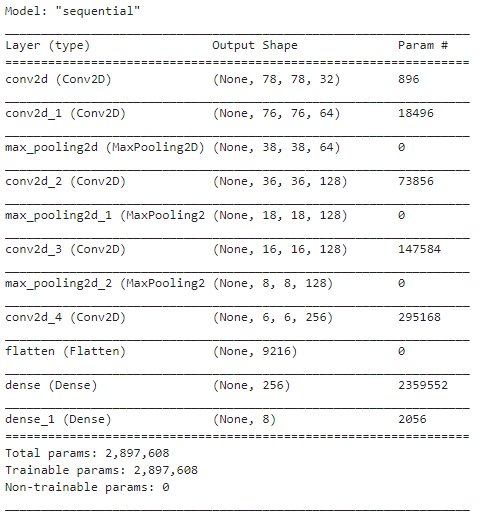
\includegraphics[width=10cm]{resources/image_model.png}
	\caption{Architecture of the model used for the images dataset.}
	\label{fig:image_model}
\end{figure}
\noindent We use Keras to build the sequential models, starting off with two convolutional layers which are made using \texttt{Conv2D} layer objects. All the \texttt{Conv2D} layers have a kernel size of $3 \times 3$. The feature map counts for the first layer is 32 and the following layer is 64. We then use a max pooling layer using the \texttt{MaxPooling2D} layer object, which reduces the size of the output by a factor of $2$ in our case where the kernel for it is of size $2 \times 2$. Max pooling layers do not learn anything new, they only propagate the highest value from its kernel window. We use the same kernel size for all \texttt{MaxPooling2D} layers. This is followed by two sets of \texttt{Conv2D} layer with a feature map count of 128 and a \texttt{MaxPooling2D} layer, in that order. We end the convolutional layers by having one last \texttt{Conv2D} layer with 256 feature maps. After that work on the classification section of the architecture. To do so, we flatten the output obtained from the last \texttt{Conv2D} layer using the \texttt{Flatten} layer and pass it to a \texttt{Dense} layer with 256 nodes. This layer is followed by the final \texttt{Dense} layer with 8 nodes which is used for the prediction of the images. The initial weights of the model are seeded as mentioned before. The compiled version of this architecture is used by the global user and federated users. We store a copy of this model in every user's User object for them to use locally. 
\subsubsection{Results}
With everything ready, we ran the first set of experiments on this dataset where the value of $P$ was $\tfrac{1}{8}$. With this, every user gets about the same number of images from every class. The experiments were ran where 32 rounds of federated learning took place with the local epoch count being 16. For the global user, the experiment ran for $32 \times 16$ epochs. 
\\\\
Once again, the graphs in Figure~\ref{fig:images_graphs_eq} show the progression of the ideas in a round-by-round manner with the $min\_max\_fill$ fill style which shades the region between the highest and the lowest evaluations. On the x-axis we have the rounds, except for Figure~\ref{fig:posture_graphs:global} where the x-axis is epochs, and on the y-axis we have the evaluations for which we used accuracy as the metric. For all the graphs, bar Figure~\ref{fig:posture_graphs:global}, the evaluations are averages of every users evaluations on their local testing data in the $pre\_fit$ and $post\_fit$ context.
\begin{figure}[H]
\centering
\begin{subfigure}{0.45\textwidth}
    \centering
    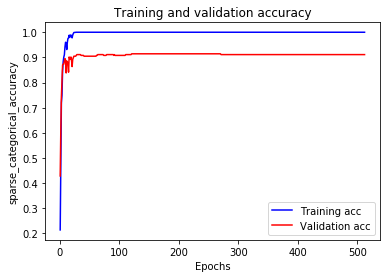
\includegraphics[width=\textwidth]{resources/posture_global_0.125-accuracy.png}
    \caption{\small Global user}

\end{subfigure}%
\\
\begin{subfigure}{0.45\textwidth}
    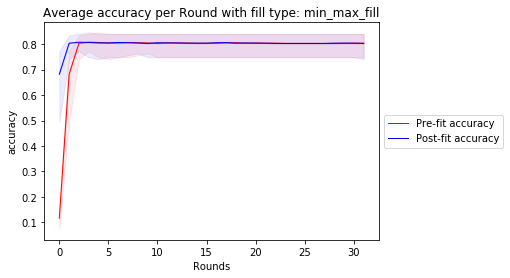
\includegraphics[width=\textwidth]{resources/posture_localround-0.125-accuracy.png}
    \raggedleft
    \caption{\small Local Training}
\end{subfigure}
\begin{subfigure}{0.45\textwidth}
    \raggedleft
    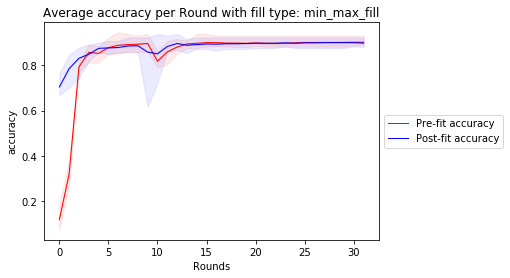
\includegraphics[width=\textwidth]{resources/posture_centralround-0.125-accuracy.png}
    \caption{\small Central Standard Averaging}
\end{subfigure}%
\\
\begin{subfigure}{0.45\textwidth}
    \raggedleft
    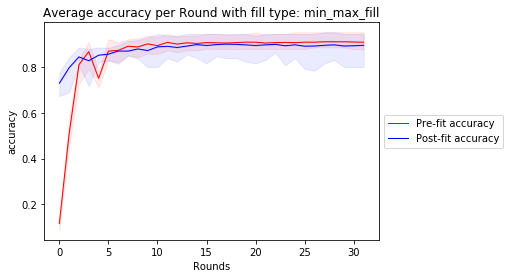
\includegraphics[width=\textwidth]{resources/posture_stdround-0.125-accuracy.png}
    \caption{Central Selective Inclusion}
\end{subfigure}
\begin{subfigure}{0.45\textwidth}
    \raggedleft
    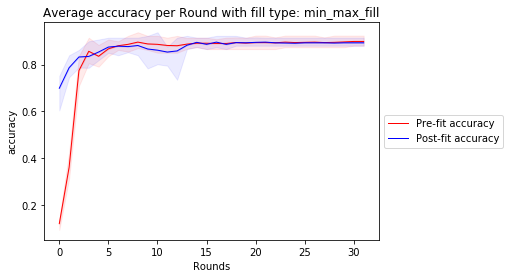
\includegraphics[width=\textwidth]{resources/posture_stdround_p2p-0.125-accuracy.png}
    \caption{Peer-to-peer Selective Inclusion}
\end{subfigure}
\\
\begin{subfigure}{0.45\textwidth}
    \raggedleft
    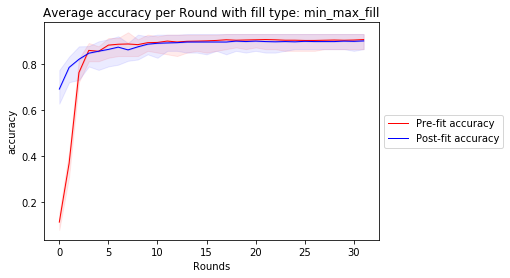
\includegraphics[width=\textwidth]{resources/posture_weightround-0.125-accuracy.png}
    \caption{Central Weighed Averaging}
\end{subfigure}
\begin{subfigure}{0.45\textwidth}
    \raggedleft
    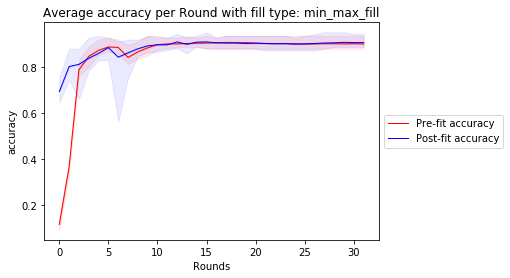
\includegraphics[width=\textwidth]{resources/posture_weightround_p2p-0.125-accuracy.png}
    \caption{Peer-to-peer Weighed Averaging}
\end{subfigure}
\caption{Graphs for the experiments on the images dataset with $P = \tfrac{1}{8}$.}\label{fig:images_graphs_eq}
\end{figure}
\noindent In this case, where everyone essentially has the same number of images for every class, we would expect the evaluations to be pretty high for all the users because they had a wide variety of images to learn from in the training process. This would result in the $min\_max\_fill$ region being very small. The graphs in Figure~\ref{fig:images_graphs_eq} show that this is indeed the case. We also see that the lower line in the fill region for the peer-to-peer ideas have a higher value than their central averaging counterpart, just as in the postures dataset. This means that once again the peer-to-peer averaging approach seems to have better models for individual users. This is further reiterated in Tables~\ref{tab:image_eq_pre_fit} and~\ref{tab:image_eq_post_fit} where we see the lowest evaluations section is higher for the peer-to-peer approaches than their central averaging counterparts. 
\begin{table}[H] % prefit -----------------------------------------------------------
\def\arraystretch{1.2}%
\resizebox{\linewidth}{!}{\begin{tabular}{|c|c|c|c|c|c|c|} %lllll
\hline
& \makecell{Local\\Training} & \makecell{Central\\Standard\\Averaging} & \makecell{Central\\Selective\\Inclusion} & \makecell{P2P\\Selective\\Inclusion} & \makecell{Central\\Weighted\\Averaging} & \makecell{P2P\\Weighted\\Averaging}\\
\hline
Average & 80.33\% & 90.18\% & 91.09\% & 89.87\% & 90.62\% & 90.19\%\\
\hline
\makecell{Standard\\Deviation} & 2.46 & 1.40 & 2.84 & 1.38 & 2.11 & 1.90\\
\hline
Lowest & 74.81\% & 88.80\% & 88.00\% & 88.06\% & 86.47\% & 88.10\%\\
\hline
Highest & 83.97\% & 93.02\% & 95.45\% & 92.37\% & 93.02\% & 93.70\%\\
\hline
\end{tabular}}
\caption{Images dataset: Pre fit results at the end of the rounds from testing user models with $P = \tfrac{1}{8}$.} \label{tab:image_eq_pre_fit}
\end{table}
\begin{table}[H] % postfit -----------------------------------------------------------
\def\arraystretch{1.2}%
\resizebox{\linewidth}{!}{\begin{tabular}{|c|c|c|c|c|c|c|} %lllll
\hline
& \makecell{Local\\Training} & \makecell{Central\\Standard\\Averaging} & \makecell{Central\\Selective\\Inclusion} & \makecell{P2P\\Selective\\Inclusion} & \makecell{Central\\Weighted\\Averaging} & \makecell{P2P\\Weighted\\Averaging}\\
\hline
Average & 80.23\% & 89.80\% & 89.74\% & 89.30\% & 90.04\% & 90.76\%\\
\hline
\makecell{Standard\\Deviation} & 2.68 & 1.39 & 4.27 & 1.27 & 1.87 & 1.95\\
\hline
Lowest & 74.05\% & 88.00\% & 80.16\% & 88.06\% & 86.47\% & 88.89\%\\
\hline
Highest & 83.97\% & 92.25\% & 94.70\% & 91.47\% & 93.02\% & 94.49\%\\
\hline
\end{tabular}}
\caption{Images dataset: Post fit results at the end of the rounds from testing user models with $P = \tfrac{1}{8}$.} \label{tab:image_eq_post_fit}
\end{table}
\noindent But the averages are essentially equal between the central and peer-to-peer approaches which means that some users from the central averaging approach are losing performance in the peer-to-peer approach. This is another trade off that might need to be discussed along with the edge user resources vs. privacy argument. It is once again dependant on the context as to whether or not a more levelled performance is better than having some very good and some very bad performing users. Although in the general case, it would seem more beneficial to have every user perform well rather than having good and bad users. 
\\\\
An interesting note here is that the local training approach is not the best one. This is probably because of the lack of shared knowledge once again. Every user has access to all the classes of images with unique images for every user. This means that the user might learn about characteristics for a class from images that another user may not have as their local data and in the federated approaches this knowledge is shared, but not in the local training idea. And this explains why the local training approach lags behind when compared to the other approaches. 
\\\\
A general note on the $pre\_fit$ and $post\_fit$ evaluations is that the averages seem to drop after the local training takes place after the weights are averaged. Even though the different is probably not significantly big, there can be an explanation behind this drop. The drop could possibly be due to the fact that the averaged weights contain more knowledge about generic characteristics on the images, and when the local training  takes place this knowledge is lost. So when we evaluate the models on unseen local test data, this cause a drop in the accuracy of the predictions. We now move on to look at how every user's model performed on the global users dataset which has more images on which the models can be evaluated. The results are seen in Table~\ref{tab:images_eq_global}.
\begin{table}[H]
\def\arraystretch{1.2}%  1 is the default, change whatever you need

\resizebox{\linewidth}{!}{\begin{tabular}{|c|c|c|c|c|c|c|c|} %lllll
\hline
 & \makecell{Non\\Federated} & \makecell{Local\\Training} & \makecell{Central\\Standard\\Averaging} & \makecell{Central\\Selective\\Inclusion} & \makecell{P2P\\Selective\\Inclusion} & \makecell{Central\\Weighted\\Averaging} & \makecell{P2P\\Weighted\\Averaging}\\
\hline
User 0 &  & 79.48\% & 91.91\% & 91.91\% & 90.94\% & 92.58\% & 91.62\%\\
\hline
User 1 &  & 79.19\% & 91.52\% & 91.71\% & 91.14\% & 92.10\% & 91.91\%\\
\hline
User 2 &  & 82.18\% & 92.10\% & 92.10\% & 90.85\% & 92.39\% & 91.71\%\\
\hline
User 3 &  & 80.15\% & 92.00\% & 92.29\% & 91.14\% & 92.29\% & 91.62\%\\
\hline
User 4 &  & 82.18\% & 91.62\% & 86.03\% & 91.52\% & 92.29\% & 91.04\%\\
\hline
User 5 &  & 81.12\% & 92.10\% & 92.68\% & 91.91\% & 91.81\% & 91.52\%\\
\hline
User 6 &  & 82.27\% & 92.29\% & 92.68\% & 91.33\% & 91.91\% & 91.81\%\\
\hline
User 7 &  & 81.21\% & 92.10\% & 92.97\% & 90.85\% & 92.29\% & 91.23\%\\
\hline
Average & 90.37\% & 80.97\% & 91.96\% & 91.55\% & 91.21\% & 92.21\% & 91.56\%\\
\hline
\end{tabular}}
\caption{Image dataset: Results from testing user models on global user's data with $P = \frac{1}{8}$} \label{tab:images_eq_global}
\end{table}
\noindent We did not expect to see a big difference here as the user's local test data was pretty representative of the whole dataset and the evaluations are indeed pretty much the same as what we saw on earlier. One thing that is added here is the evaluation from the non-federated approach of the global user. We can see that the averages from all the ideas, bar local training, are in-fact higher than that of the non-federated approach. This could be due to chance or due to the fact that the model started over-fitting after being exposed to the same data for too long, although the learning curve from Figure~\ref{fig:images_graphs_eq} does not suggest this. So it is very likely that this is due to chance and that their performance is essentially the same on the global user's test data.
\\\\
The experiment with $P=\frac{1}{8}$ was interesting because of the almost equal split of data amongst all the users. But this would rarely be the case in a real world scenario where a user is probably more biased to taking pictures of a certain class. To simulate this situation, we changed the value of $P$ to be $0.7$. This means that every user is biased to having more pictures of a certain class when compared to the others. More specifically, almost 70\% of a user's data would be images from a specific class, and the rest would be a split from the remaining classes. Almost every user gets at least one images from every class in this part of the experiment. This was once again ran for 32 rounds of federated learning for 16 epochs and the global user's experiment ran for $32 \times 16$ epochs. The graphs from these experiments can be seen in Figure~\ref{fig:images_graphs_biased}.
\begin{figure}[H]
\centering
\begin{subfigure}{0.45\textwidth}
    \centering
    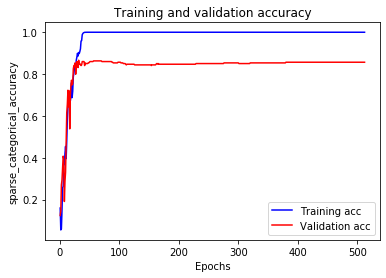
\includegraphics[width=\textwidth]{resources/posture_global_0.7-accuracy.png}
    \caption{\small Global user}

\end{subfigure}%
\\
\begin{subfigure}{0.45\textwidth}
    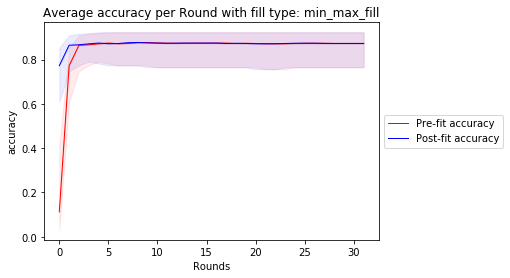
\includegraphics[width=\textwidth]{resources/posture_localround-0.7-accuracy.png}
    \raggedleft
    \caption{\small Local Training}
\end{subfigure}
\begin{subfigure}{0.45\textwidth}
    \raggedleft
    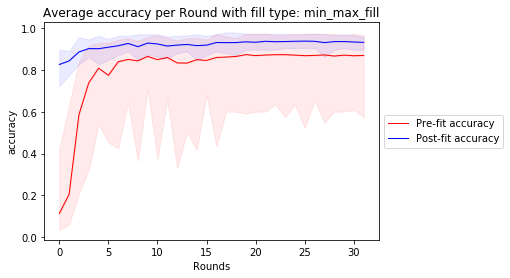
\includegraphics[width=\textwidth]{resources/posture_centralround-0.7-accuracy.png}
    \caption{\small Central Standard Averaging}
\end{subfigure}%
\\
\begin{subfigure}{0.45\textwidth}
    \raggedleft
    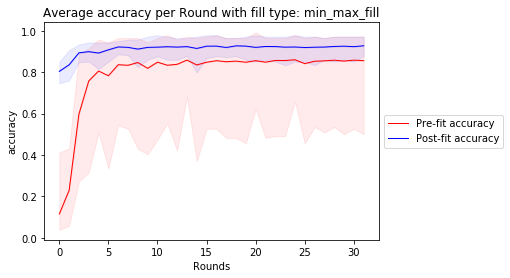
\includegraphics[width=\textwidth]{resources/posture_stdround-0.7-accuracy.png}
    \caption{Central Selective Inclusion}
\end{subfigure}
\begin{subfigure}{0.45\textwidth}
    \raggedleft
    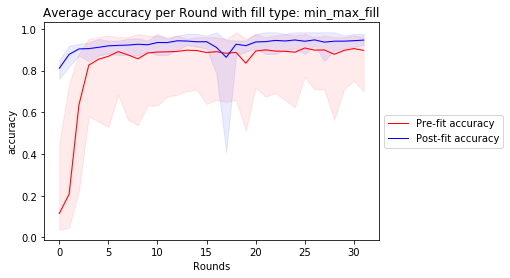
\includegraphics[width=\textwidth]{resources/posture_stdround_p2p-0.7-accuracy.png}
    \caption{Peer-to-peer Selective Inclusion}
\end{subfigure}
\\
\begin{subfigure}{0.45\textwidth}
    \raggedleft
    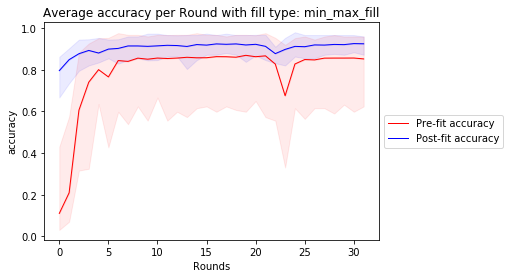
\includegraphics[width=\textwidth]{resources/posture_weightround-0.7-accuracy.png}
    \caption{Central Weighed Averaging}
\end{subfigure}
\begin{subfigure}{0.45\textwidth}
    \raggedleft
    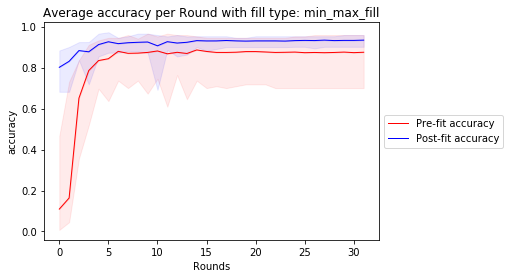
\includegraphics[width=\textwidth]{resources/posture_weightround_p2p-0.7-accuracy.png}
    \caption{Peer-to-peer Weighed Averaging}
\end{subfigure}
\caption{Graphs for the experiments on the images dataset with $P = 0.7$.}\label{fig:images_graphs_biased}
\end{figure}
\noindent We can see that the graphs have a bit more of the fill region for the $pre\_fit$ line which shows that the averaged weights are not the best set of weights for the local test data of some users. This is probably because the averaging process causes a loss of knowledge of the user's image bias. The global user's learning curve does not show any signs of over-fitting from its learning curve, just like the other experiment. And once again, as has been the case with all other experiments, the lower bound of the filling region for the $pre\_fit$ line is higher for the peer-to-peer approaches than the that of their central averaging counterparts and Tables~\ref{tab:image_biased_pre_fit} and~\ref{tab:image_biased_post_fit} support that as well. Other than that, they are all performing at essentially the same level as each other. The local training idea seems to be performing better as a whole considering its smaller fill region but the better evaluation will be when we test it on the global user's test data later.
\begin{table}[H] % prefit -----------------------------------------------------------
\def\arraystretch{1.2}%
\resizebox{\linewidth}{!}{\begin{tabular}{|c|c|c|c|c|c|c|} %lllll
\hline
& \makecell{Local\\Training} & \makecell{Central\\Standard\\Averaging} & \makecell{Central\\Selective\\Inclusion} & \makecell{P2P\\Selective\\Inclusion} & \makecell{Central\\Weighted\\Averaging} & \makecell{P2P\\Weighted\\Averaging}\\
\hline
Average & 87.31\% & 86.84\% & 85.58\% & 89.72\% & 85.18\% & 87.49\%\\
\hline
\makecell{Standard\\Deviation} & 4.41 & 11.64 & 13.90 & 7.87 & 11.21 & 7.45\\
\hline
Lowest & 76.52\% & 57.39\% & 50.00\% & 70.09\% & 62.39\% & 70.00\%\\
\hline
Highest & 92.36\% & 96.53\% & 97.16\% & 96.03\% & 95.90\% & 95.89\%\\
\hline
\end{tabular}}
\caption{Images dataset: Pre fit results at the end of the rounds from testing user models with $P = 0.7$.} \label{tab:image_biased_pre_fit}
\end{table}
\begin{table}[H] % postfit -----------------------------------------------------------
\def\arraystretch{1.2}%
\resizebox{\linewidth}{!}{\begin{tabular}{|c|c|c|c|c|c|c|} %lllll
\hline
& \makecell{Local\\Training} & \makecell{Central\\Standard\\Averaging} & \makecell{Central\\Selective\\Inclusion} & \makecell{P2P\\Selective\\Inclusion} & \makecell{Central\\Weighted\\Averaging} & \makecell{P2P\\Weighted\\Averaging}\\
\hline
Average & 87.31\% & 93.11\% & 92.76\% & 94.66\% & 92.45\% & 93.41\%\\
\hline
\makecell{Standard\\Deviation} & 4.41 & 2.35 & 2.90 & 1.40 & 3.04 & 1.65\\
\hline
Lowest & 76.52\% & 89.57\% & 87.72\% & 92.31\% & 87.18\% & 90.15\%\\
\hline
Highest & 92.36\% & 95.83\% & 97.16\% & 97.62\% & 95.95\% & 95.89\%\\
\hline
\end{tabular}}
\caption{Images dataset: Post fit results at the end of the rounds from testing user models with $P = 0.7$.} \label{tab:image_biased_post_fit}
\end{table}
\noindent From the two tables we can see that the local training helps out the users not performing well on the averaged weights as the lowest evaluations rise sharply in Table~\ref{tab:image_biased_post_fit} which is for the $post\_fit$ evaluations. The same trend of the peer-to-peer idea being better for individual users is seen here with the higher lowest evaluations, higher averages and lower standard deviations as seen in both tables. This made us more confident in saying that the peer-to-peer approach increases the privacy by decentralising the process and gives better performance for individual users. Other than the peer-to-per ideas, the central averaging ideas seem to be performing pretty much on the same level as each other.
\begin{table}[H]
\def\arraystretch{1.2}%  1 is the default, change whatever you need

\resizebox{\linewidth}{!}{\begin{tabular}{|c|c|c|c|c|c|c|c|} %lllll
\hline
 & \makecell{Non\\Federated} & \makecell{Local\\Training} & \makecell{Central\\Standard\\Averaging} & \makecell{Central\\Selective\\Inclusion} & \makecell{P2P\\Selective\\Inclusion} & \makecell{Central\\Weighted\\Averaging} & \makecell{P2P\\Weighted\\Averaging}\\
\hline
User 0 &  & 77.31\% & 89.42\% & 88.08\% & 89.52\% & 88.27\% & 88.08\%\\
\hline
User 1 &  & 73.37\% & 88.65\% & 87.98\% & 86.73\% & 87.50\% & 88.75\%\\
\hline
User 2 &  & 71.54\% & 87.69\% & 87.12\% & 88.17\% & 85.58\% & 85.67\%\\
\hline
User 3 &  & 73.46\% & 88.94\% & 87.12\% & 86.54\% & 87.88\% & 88.27\%\\
\hline
User 4 &  & 66.35\% & 76.44\% & 77.40\% & 78.65\% & 80.87\% & 80.10\%\\
\hline
User 5 &  & 74.04\% & 89.52\% & 88.17\% & 89.23\% & 88.17\% & 88.75\%\\
\hline
User 6 &  & 74.04\% & 88.94\% & 87.88\% & 88.85\% & 87.88\% & 88.46\%\\
\hline
User 7 &  & 66.06\% & 81.35\% & 84.13\% & 83.65\% & 81.54\% & 82.31\%\\
\hline
Average & 87.21\% & 72.02\% & 86.37\% & 85.99\% & 86.42\% & 85.96\% & 86.30\%\\
\hline
\end{tabular}}
\caption{Image dataset: Results from testing user models on global user's data with $P = 0.7$}\label{tab:images_biased_global}
\end{table}
\noindent We now look at the evaluations of the user's models on the global user's testing data shown in Table~\ref{tab:images_biased_global}. As expected, the accuracies shown here are lower than the ones in Tables~\ref{tab:image_biased_pre_fit} and~\ref{tab:image_biased_post_fit} because they were conducted on the user's local test data which is biased towards the user's overall dataset. The global user's more varied test data means that the results are more objective in terms of the performance. The local training idea is the worst performing idea once again because of the lack of shared knowledge it could have gained from a federated approach. Even though it is the idea which provides the utmost privacy, the performance loss seen in it is too much on the more generic dataset. Again, depending on the context, this might be acceptable but in the general case it is more desirable to have a model that can predict well on a wider range of samples.
\\\\
Other than the local training idea, the other ideas are once again performing on pretty much the same level and even almost matching the non-federated learning idea. This means that we can say with confidence that the federated learning ideas are very close to the performance of the non-federated approach but provide more privacy. The peer-to-peer ideas further build up on that idea more and provide even more privacy whilst maintaining the same level of overall performance. The higher level of privacy is gained by decentralising the process but at the cost of more computations to be done on the edge users. It even provides a more levelled out performance across all the users, as seen from the experiments with the lower standard deviations and higher values for the lowest evaluations seen per round for any given user.
\\\\
With the experimentation process and their results discussed, we move on to the final section where we talk about our concluding remarks on this project and further work that can be done in this area. We will also discuss things that could have been done better or differently in this project. 
%\subsubsection{Testing user weights on global data}
\clearpage
\section{Conclusions and future work}
We started this report by looking at what machine learning is and how neural networks work. After doing so, we introduced the idea of federated learning which is a distributed form of training a neural network. In federated learning, every user trains a local model and then the weights from the models are averaged by a central agent and sent back to the users. This way the user's privacy is maintained and the knowledge from other users' models is incorporated into every user's model. We then introduced several extensions to this in the form of weighted averaging, where better performing models are weighted higher in the averaging process, and selective inclusion where certain user's are excluded from the averaging process based on their performance. These extensions were also then implemented in a peer-to-peer context where user's conduct weighted averaging and selective inclusion based on how well other users' models perform on their local data. The idea of localised training, where users do not share their weights at all, was also implemented. These ideas were then compared by running three sets of experiments on two different datasets. The main aim was to see if the extended provided a performance gain or if they provided more privacy at relatively the same performance.
\\\\
As seen from all the experiments that were conducted, none of the extended ideas resulted in a significant gain in overall performance when compared to Google's original idea of federated learning. But, the points raised earlier about the peer-to-peer approach providing a bit more privacy and more levelled out performance across all the users were quite interesting in my opinion. I believe that this is quite a significant find that needs to be explored further and more experiments need to be carried out for the same. With the edge devices getting more powerful by the day, it seems more and more viable that the decentralised peer-to-peer federated learning approach could be the future. In theory, it makes a lot of sense to me and the experiments showed great promise in the idea as well. One of its shortcomings was the fact that some user's seemed to be getting lower performance with it, but that could be a dataset specific characteristic. Maybe with models made specifically for a federated learning environment, it could do better overall as well. So I think that the peer-to-peer federated learning approach needs to be further explored in the future because of the promise it shows.
\\\\
In this project, I did not implement the idea of early stopping for the training which would probably help improve the performance. This is where the user's can stop training their model if its performance gets lower after a few epochs, and they would then revert the model back to its best performing state. This could have helped increase the overall performance for all the approaches. It's effect would have been interesting to note in the experiments. Another thing that could have been done is the sharing of deltas in the weights instead of the weights themselves. In a real world scenario, this would help reduce the bandwidth required to perform federated learning. Albeit very unlikely, it could have also had an effect on the performance of the all the federated learning ideas that were implemented. 
\\\\
The idea of secure aggregation when collecting the weights could also have been implemented and explored to see what, if any, effect it had on the federated learning ideas that were implemented in this project. The final thing that could have been done for more credible results was to have a framework that would report results from running the experiments several times and then reporting the averages from all those experiments. The results would have been more robust and more reliable this way, and a relatively small tweak to the testing framework can easily make this possible. 
\comment{
	summary
	conclusions from work
		what does the project contribute to the human knowledge 
	future developments or line of eqnuiry suggested by the work
}
\subsection{Reflection}
Throughout the course of this project, I got a better understanding of how neural networks work and details on how the underlying algorithms work. Working on this project required a lower level understanding of neural network and this knowledge was gained from the book "Deep Learning with Python"~\cite{deeplearning}. Knowledge on how to work with Keras well was also gained from the same book to the point where I can say that I am fairly comfortable using Keras. I do not know everything but I know enough to get started and work my way through things now. 
\\\\
Early on when I first started working on this project, I was overwhelmed by the work that was to be done and because of that I was not making good progress. But after setting realistic weekly goals, I started making steady progress and eventually started flying through the list of things that needed to be done. So organising myself was key in this process. The same applied to the code structure. I had to restructure and rewrite a lot of the code because I was not happy with how it was implemented at the start. Taking some time to work out the structure beforehand and not hacking away at the code proved to be more beneficial in the long term. 
\subsection{Project Timeline}
\comment{
	reglection subsection
		what did I learn, new skills, short comings (skill, method, time)
	summary of project conduction
		timeline 
}
In terms of the overall time aspect of this project, I believe I handled it relatively well. I started working on the project as soon as it was assigned to me in September, 2019. The first task to complete was to read the background information on the project, which included reading the paper on federated learning by Google~\cite{mcmahan2016communication} and the deep learning book~\cite{deeplearning} which was done in two weeks times. After that, I started building a model for the postures dataset for the non-federated approach and then eventually building the federated learning approach as Google does it. This took a total of two weeks. Then, to visually report on the experiments, I implemented the graphing framework. I also refactored a lot of code at this point for better structuring and some bug fixing which took about one week.
\\\\
After the basics were done, the extended ideas ideas were implemented for the next three weeks. And at the end, one week before the start of November, all the ideas and the implementation of the ideas was completed. My main aim was to finish implementation aspect of the project by the end of October so that I had time to study for the exams. It was an ambitious goal, but it was met in the end. In the last week, I spent time going over the TensorFlow documentation and seeing if my implementation was the same as the implementation in TensorFlow Federated. After that, the next time I worked on it was when college started in the second week of January. It was a bit unfortunate that I did not work on the project over the Christmas break, but it was not a big issue because I had quite a lot of my work done. I only read a paper on secure aggregation over the break.
\\\\
For the first week we were back to college in January, I worked on making TensorFlow Federated work the the postures dataset. The next three weeks were spent on implementing the local training idea and an experimentation framework to report the results. There was a delay here because of the memory limitations not allowing us to run everything in one go elegantly. After I was unable to find an elegant solution, I chose to use swap space as a workaround for the limitation. Another thing was was worked on during these three weeks is the work required for the images datasets. The implementation of the splitting strategy and everything associated with running experiments on this dataset. At this point it was about the middle of February, at which point I stopped coding and started focussing on the report with only minor fixes and adjustments of the code. The report writing lasted for about two months, which brings here to this point here, at the end.
\comment{
	basic thing
	read book
	google implementation
	better graphinh 
	extended ideas
	repreodcuible
	testing
	results
	report - 2 months 
}
\clearpage
\printbibliography[title={Bibliography}]
\end{document}

